\documentclass{ltjsarticle}

\usepackage{fontspec}
\usepackage{luatexja-fontspec} % ltjsarticle なら必要

\usepackage{jlcode}


\usepackage{xcolor}

\usepackage{amsmath,amssymb,mathtools,bm,physics}
\mathtoolsset{showonlyrefs=true}
\usepackage{luacas}
\usepackage{graphicx,here,tikz}
\usepackage{hyperref}
\title{厳密対角化}
\author{1222031 北野志}
\date{\today}

\begin{document}
\maketitle
\section{量子力学の基本的な計算を目的としたコード}
\subsection*{コードの構成}
\begin{jllisting}
module ExactDiag
const _dim = Ref(1)
const _site = Ref(1)
const _trans = Ref(Vector{Vector{Int}}())  
const _reverse = Ref(Dict{Vector{Int}, Int}()) 
export # ここに外でも使う関数を列挙する
end
\end{jllisting}
基本的には上のようにmoduleを定義してその中で関数を定義していく。(毎回関数に各サイトの次元\_dimとサイト数\_siteとFock状態の番号を渡すのは面倒なため)\\
\subsection*{用いるパッケージ}
\begin{jllisting}
using LinearAlgebra
using PrettyTables
using SparseArrays
using UnionFind
\end{jllisting}
厳密対角化ではいくつかの線形代数の関数を用いるためLinearAlgebraを、メモリの消費量を減らすのを目的として行列のスパース表現を用いるためSparseArraysを、行列の表示をきれいにするためPrettyTablesを、UnionFindはブロック対角化のために用いる。\\
\subsection*{初期化の関数}
\begin{jllisting}
function init(dim::Int, site::Int)
  _dim[] = dim
  _site[] = site
  dim_tot = dim^site
  _trans[]=Vector{Vector{UInt8}}(undef, dim_tot)
  row = zeros(Int, site)
  _trans[][1] = copy(row)
  @inbounds for i in 1:dim_tot-1
    j = site
    while true
      v = row[j] + 1
      if v == dim
        row[j] = 0
        j -= 1
      else
        row[j] = v
        break
      end
    end
    _trans[][i+1] = copy(row)
  end
  _reverse[] = Dict{Vector{Int}, Int}(_trans[][i] => i for i in eachindex(_trans[]))
end
\end{jllisting}
各サイトの次元\_dim(スピンの大きさ$s$として、$2s+1$)とサイト数\_siteを指定して初期化する。\\
さらに加えて、Fock状態の番号付けを行うための配列\_ reverseとその逆変換を行うための配列\_transとを定義する。(メモしておくことで計算量を削減できる)\\
\subsection*{Fock状態の番号付け}
\begin{jllisting}
function Nary_reverse(n::Vector{Int})
  if haskey(_reverse[], n)
    return copy(_reverse[][n])
  elseif length(n)!=_site[]
    throw(ArgumentError("n must be a vector of length site"))
  else
    throw(ArgumentError("n is not a valid state"))
  end
end
\end{jllisting}
この関数は、Fock状態を\_site進数で表現したときの整数値を1-indexで返すことにより番号付けしている。\\
たとえば、サイト数が3で次元が2のとき、状態$\ket{001}$は$1+0\cdot 2^2 + 0\cdot 2^1 + 1\cdot 2^0 = 2$、$\ket{101}$は$1+1\cdot 2^2 + 0\cdot 2^1 + 1\cdot 2^0 = 6$となる。\\
\begin{jllisting}
function Nary_trans(t::Int)
  if t == 0
    return [-1 for _ in 1:_site[]]
  elseif t < 1 || t > _dim[]^_site[]
    throw(ArgumentError("t must be in the range [0, dim^site - 1]"))
  else
    return copy(_trans[][t])
  end
end
\end{jllisting}
逆に整数値からFock状態の表示に戻す。\\
引数が0だとすべてのサイトが-1を返す仕様である。(変更の可能性あり)\\
\subsection*{関数の定義とその演算}
\begin{jllisting}
struct Op
  op::Vector{Tuple{ComplexF64,Vector{Function}}}
  function Op(op::Vector{Tuple{ComplexF64,Vector{Function}}})
    new(op)
  end
  function Op(op1::Function)
    vecf = Vector{Function}([op1])
    Op([(1.0 + 0.0im, vecf)])
  end
end 
\end{jllisting}
このように演算子を定義する。Vector\{Function\}はその要素であるFunctionの積を表しており、Tuple\{ComplexF64,Vector\{Function\}\}のComplexF64がVector\{Function\}の係数を表しており、Vector\{Tuple\{ComplexF64,Vector\{Function\}\}\}の要素であるTuple\{ComplexF64,Vector\{Function\}\}の総和を表している。\\
例えば、Functionとして$A,B,C,D,E$を定義すると
$\{(1.0+0.0i,\{A,B\}),(1.5+0.0i,\{C,D\}),(0.5+0.0i,\{E\})\}$は$AB+1.5CD+0.5E$を表している。
\begin{jllisting}
import Base: *, +, -, show, sum
\end{jllisting}
演算子に用いる記号のオーバーロードを行う。
\begin{jllisting}
function +(ops::Op...)
  k = Vector{Tuple{ComplexF64,Vector{Function}}}()
  for op1 in ops
    k = vcat(k, op1.op)
  end
  Op(k)
end
\end{jllisting}
演算子同士の足し算は演算子のベクトルを連結することで定義する。
\begin{jllisting}
function *(op1::Op)
  op1
end
function *(op1::Op, op2::Op...)
  op3 = *(op2...)
  k = Vector{Tuple{ComplexF64,Vector{Function}}}()
  for op11 in op1.op
    for op31 in op3.op
      push!(k, (op11[1] * op31[1], vcat(op11[2], op31[2])))
    end
  end
  Op(k)
end
\end{jllisting}
演算子同士の掛け算は分配法則を用いて帰納的に定義されている。
\begin{jllisting}
function *(coeff::Union{ComplexF64,Float64}, op1::Op...)
  op2 = *(op1...)
  k = Vector{Tuple{ComplexF64,Vector{Function}}}()
  for op21 in op2.op
    push!(k, (op21[1] * ComplexF64(coeff), op21[2]))
  end
  Op(k)
end
\end{jllisting}
通常の数(自前で書くときに面倒なので複素数と実数どちらでも良くしている)と演算子の掛け算は係数にその数を掛けることによって定義されている。\\
\begin{jllisting}
function *(op1::Op, t::Int)
  t1 = copy(t)
  for op11 in op1.op[1][2]
    t1 = op11(t1)[2]
  end
  sum = 0.0 + 0.0im
  for op11 in op1.op
    product = op11[1]
    t2 = copy(t)
    for op12 in op11[2]
      t2 = op12(t2)[2]
      product *= op12(t2)[1]
    end
    if t2 != t1
      throw(ArgumentError("The operator does not preserve the state."))
    end
    sum += product
  end
  return (sum, t1)
end
\end{jllisting}
整数で表されるFock状態に対して演算子を作用させる。\\
この場合は、作用させた後に単一のFock状態に戻る場合のみに用いることができる。(そうでなければエラーが出る仕様)
\begin{jllisting}
function -(op1::Op)
  (-1.0 + 0.0im) * op1
end
function -(op1::Op, op2::Op)
  op1 + (-op2)
end
function -(op1::Op, op2::Op...)
  op3 = +(op2...)
  op1 - op3
end
\end{jllisting}
演算子同士の引き算は通常の数との積を用いて帰納的に定義されている。
\begin{jllisting}
function sum(mat::Op)
  return mat
end
function sum(op1::Op, op2::Op...)
  op3 = sum(op2...)
  ans = op1 + op3
  return ans
end
function sum(f::Function, k::Int=0)
  sum(Tuple(f(i) for i in k:(_site[]-1))...)
end
\end{jllisting}
演算子の和を計算する関数であり、引数の演算子の総和を求められる。\\
下の関数の適用例として
\begin{jllisting}
sum(i->f(i))
\end{jllisting}
上のように表記することで、サイト数で総和の範囲を指定することもできる。\\
\begin{jllisting}
sum(i->f(i), k)
\end{jllisting}
上のように表記することで、kから最後までの総和を求めることもできる。(開放端条件などのために用いられる)\\
\subsection*{具体的な演算子の定義}
作用させた後に単一のFock状態に戻る演算子のみを定義する。\\
\begin{jllisting}
function id(i::Int)
  if i < 1 || i > _dim[]^_site[]
    throw(ArgumentError("i must be in the range [1, dim^site]"))
  end
  return (1.0 + 0.0im, i)
end
id() = Op(id)
\end{jllisting}
恒等演算子はFock状態をそのまま係数1で返すと定義されている。(範囲外の場合はエラーが出る)
\begin{jllisting}
function shift(k::Int=1)
  function shift1(t::Int)
    n = Nary_trans(t)
    n1 = circshift(n, k)
    return (1.0 + 0.0im, Nary_reverse(n1))
  end
  return Op(shift1)
end
\end{jllisting}
並進演算子はFock状態を$k$だけ右にずらすと定義されている。(デフォルトでは1だけずらす)\\
\begin{jllisting}
function site_flip(t::Int)
  n = Nary_trans(t)
  n1 = reverse(n)
  return (1.0 + 0.0im, Nary_reverse(n1))
end
site_flip() = Op(site_flip)
\end{jllisting}
サイト反転演算子はFock状態を反転させると定義されている。\\
\begin{jllisting}
function spin_flip(t::Int)
  n = Nary_trans(t)
  n1 = Vector{Int}(undef, _site[])
  for i in 1:_site[]
    n1[i] = _dim[]/2.0 - n[i]
  end
  return (1.0 + 0.0im, Nary_reverse(n1))
end
spin_flip() = Op(spin_flip)
\end{jllisting}
スピン反転演算子はFock状態の各サイトのスピンを反転させると定義されている。(スピンの大きさが1/2の場合のみ定義されている)\\
\begin{jllisting}
function spin(kind::Char, site::Int)
  site_number = _site[]
  idx = mod(site-1,site_number)+1
  if kind == '+'
    plus = function (t::Int)
      n = Nary_trans(t)
      n[idx] += 1
      return n[idx] < _dim[] ? (1.0 + 0im, Nary_reverse(n)) : (0.0 + 0im, t)
    end
    return Op(plus)
  elseif kind == '-'
    minus = function (t::Int)
      n = Nary_trans(t)
      n[idx] -= 1
      return n[idx] > -1 ? (1.0 + 0im, Nary_reverse(n)) : (0.0 + 0im, t)
    end
    return Op(minus)
  elseif kind == 'x'
    plus = function (t::Int)
      n = Nary_trans(t)
      n[idx] += 1
      n[idx] < _dim[] ? (1.0 + 0im, Nary_reverse(n)) : (0.0 + 0im, t)
    end
    minus = function (t::Int)
      n = Nary_trans(t)
      n[idx] -= 1
      n[idx] > -1 ? (1.0 + 0im, Nary_reverse(n)) : (0.0 + 0im, t)
    end
    return 0.5 * (Op(plus) + Op(minus))
  elseif kind == 'y'
    plus = function (t::Int)
      n = Nary_trans(t)
      n[idx] += 1
      n[idx] < _dim[] ? (1.0 + 0im, Nary_reverse(n)) : (0.0 + 0im, t)
    end
    minus = function (t::Int)
      n = Nary_trans(t)
      n[idx] -= 1
      n[idx] > -1 ? (1.0 + 0im, Nary_reverse(n)) : (0.0 + 0im, t)
    end
    return (-0.5im) * (Op(plus) - Op(minus))
  elseif kind == 'z'
    z = function (t::Int)
      n = Nary_trans(t)
      ((_dim[] - 1.0) / 2.0 - n[idx] + 0.0im, t)
    end
    return Op(z)
  else
    throw(ArgumentError("kind must be '+', '-', 'x', 'y', or 'z'"))
  end
end
\end{jllisting}
スピン演算子はスピンの種類とサイト番号を指定して定義される。\\
スピンの種類は$+$, $-$, $z$, $x$, $y$の5種類がある。\\
スピンの種類$+$はスピンを1つ上げる演算子、$-$はスピンを1つ下げる演算子、$z$はスピンのz成分を返す演算子、$x$はスピンを1つ上げる演算子と1つ下げる演算子の和の半分、$y$はスピンを1つ上げる演算子と1つ下げる演算子の差の虚数倍の半分である。(普通に関数を定義するとエラーが出るので、無名関数を用いて定義しておく)\\
\begin{jllisting}
function num(site::Int)
  number = function (t::Int)
    n = Nary_trans(t)
    return (n[site] + 0.0im, t)
  end
  return Op(number)
end
\end{jllisting}
Jordan-Wigner変換を用いて、スピンのz成分を数演算子に変換するための関数である。\\
\begin{jllisting}
function S_z()
  return sum(j->spin('z', j))
end
\end{jllisting}
スピンのz成分を全てのサイトに対して和を取った演算子である。\\
\subsection*{ハミルトニアンの行列とその表示}
\begin{jllisting}
function matrix(op1::Union{Matrix{ComplexF64},Op})
  if isa(op1, Matrix{ComplexF64})
    return op1
  end
  dimention = _dim[]
  site_number = _site[]
  dim_tot = dimention^site_number
  mat = zeros(ComplexF64, dim_tot, dim_tot)
  for t in 1:dim_tot
    for (coeff, op11) in op1.op
      t1 = t
      coeff1 = coeff
      for op12 in op11
        (v1, t1) = op12(t1)
        coeff1 *= v1
      end
      mat[t, t1] += coeff1
    end
  end
  return mat
end
\end{jllisting}
ハミルトニアンの行列を計算する関数であり、それぞれの演算子要素ごとに関数を作用させていってゼロ行列に加えていくことで行列が生成される。\\
\begin{jllisting}
function complex_formatter(; digits::Int=1)
  return (v, i, j) -> begin
    if v == 0 + 0im
      @sprintf("%.*f", digits, 0.0)
    elseif isa(v, Complex)
      rea = round(real(v), digits=digits)
      image = round(imag(v), digits=digits)
      if image == 0
        @sprintf("%.*f", digits, rea)
      elseif rea == 0
        @sprintf("%.*fim", digits, image)
      else
        sign = image > 0 ? "+" : "-"
        @sprintf("%.*f%s%.*fim", digits, rea, sign, digits, abs(image))
      end
    elseif isa(v, Number)
      @sprintf("%.*f", digits, v)
    else
      string(v)
    end
  end
end
\end{jllisting}
複素数を指定した桁数で表示させるためのフォーマットであり、行列の表示に用いられる。中身はよくわかっていない。\\
\begin{jllisting}
function show(op1::Op, digit::Int=1)
  mat1 = matrix(op1)
  pretty_table(mat1, header=([join(string.(Nary_trans(i)), "") for i in 1:size(mat1, 1)]), row_labels=([join(string.(Nary_trans(i)), "") for i in 1:size(mat1, 2)]), formatters=complex_formatter(digits=digit))
end
\end{jllisting}
Fock状態による行列を表示できる関数である。(デフォルトで小数点以下1桁表示)\\
\begin{jllisting}
function show_eigens(vec1::Vector{Float64},mat1::Matrix{ComplexF64}, digit::Int=1)
  mat2=transpose(mat1)
  pretty_table(mat2, header=([join(string.(Nary_trans(i)), "") for i in 1:size(mat1, 1)]), row_labels=([string(vec1[i]) for i in 1:size(mat1, 2)]), formatters=complex_formatter(digits=digit))
end
\end{jllisting}
固有エネルギーと固有状態を表示する関数である。(デフォルトで小数点以下1桁表示)\\
\subsection*{代表的なハミルトニアンの表示}
これまでの演算子の関数を用いて代表的なハミルトニアンを表示してみる。\\
まず、初期化をしておく。
\begin{jllisting}
init(2, 4)
\end{jllisting}
スピン$\frac{1}{2}$の4サイトの系を考える。\\
横磁場イジング模型(周期境界条件)
\begin{align}
  H = \sum_{j=1}^{L} \left( S^z_j S^z_{j+1} - h S^x_{j} \right)
\end{align}
このハミルトニアンは$J$を用いて無次元化して
\begin{jllisting}
hj = 2.0
H1 = sum(j -> spin('z', j) * spin('z', j + 1) - hj * spin('x', j))
\end{jllisting}
と表せる。(hjは縦磁場の強さを表す$\frac{h}{J}$であるがどんな値でもよい)\\
開放端条件ならば
\begin{align}
  H = \sum_{j=1}^{L-1} S^z_j S^z_{j+1} - h \sum_{j=1}^{L} S^x_{j}
\end{align}
\begin{jllisting}
H1 = sum(j -> spin('z', j) * spin('z', j + 1), 1) - sum(j -> hj * spin('x', j))
\end{jllisting}
と表される。\\
XXZ模型(周期境界条件)
\begin{align}
  H = \sum_{j=1}^{L} \left( S^x_j S^x_{j+1} + S^y_j S^y_{j+1} + \Delta S^z_j S^z_{j+1} \right)
\end{align}
\begin{jllisting}
Δ = 2.0
H2 = sum(j -> spin('x', j) * spin('x', j + 1) + spin('y', j) * spin('y', j + 1) + Δ * spin('z', j) * spin('z', j + 1))
\end{jllisting}
と表せる。\\
開放端条件ならば
\begin{align}
  H = \sum_{j=1}^{L-1} \left( S^x_j S^x_{j+1} + S^y_j S^y_{j+1} + \Delta S^z_j S^z_{j+1} \right)
\end{align}
\begin{jllisting}
H2 = sum(j -> spin('x', j) * spin('x', j + 1) + spin('y', j) * spin('y', j + 1) + Δ * spin('z', j) * spin('z', j + 1), 1)
\end{jllisting}
と表される。\\
Bose-Hubbard模型(開放端条件)
\begin{align}
  H &= -J\sum_{j=1}^{L-1} \left( a_j^\dagger a_{j+1} + a_{j+1}^\dagger a_j \right) + \frac{U}{2}\sum_{j=1}^{L} n_j(n_j-1)
\end{align}
\begin{jllisting}
Uj = 2.0
H3 = sum(j -> -spin('+', j) * spin('-', j + 1) - spin('-', j) * spin('+', j + 1), 1) + sum(j -> (Uj / 2.0) * num(j) * (num(j) - 1.0 * id()))
\end{jllisting}
と表せる。(Jordan-Wigner変換を用いている)\\
Bose-Hubbard模型においては周期境界条件でJordan-Wigner変換を用いると非自明な項が出てくるため、開放端条件で定義している。\\
\section{固有状態とそれを基底としたハミルトニアンの計算方法}
ここでは少し一般の系を扱う。
\subsection{無限の場合の固有状態}
$\hat{A}$と任意の状態$\ket{\varphi}$について\\
固有値$\alpha$の固有状態$\ket{\alpha}$は
\begin{align}
  \ket{\alpha}=C\sum_{n=-\infty}^{\infty} \left(\frac{\hat{A}}{\alpha} \right)^n \ket{\varphi}
\end{align}
と表せる。($C$は規格化係数)\\
ここで、$\hat{A}^{-n}\ket{\varphi}$($n\ge0$)は$\ket{\varphi}=\hat{A}^0\ket{\varphi}$であり、$n=k$として$\hat{A}^{-k}\ket{\varphi}$が定義された場合に状態$\hat{A}^{-(k+1)}\ket{\varphi}$は、$\hat{A}^{-k}\ket{\varphi}=\hat{A}(\hat{A}^{-(k+1)}\ket{\phi})$を満たすとして、再帰的に定義する。(一意に決まるかどうかはわからないが、定義を満たす状態を用いればよい)\\
ただし、$\norm{\ket{\alpha}}<\infty$とする。\\
\subsubsection*{証明}
\begin{align}
  \hat{A}\ket{\alpha} &= C\sum_{n=-\infty}^{\infty} \alpha^{-n} \hat{A}^{n+1} \ket{\varphi}\\
  &= C\sum_{n=-\infty}^{\infty} \alpha^{-n+1} \hat{A}^{n} \ket{\varphi}\\
  &= \alpha C\sum_{n=-\infty}^{\infty} \left(\frac{\hat{A}}{\alpha} \right)^{n} \ket{\varphi}\\
  &= \alpha \ket{\alpha}
\end{align}
\subsubsection*{具体例}
調和振動子について、消滅演算子$\hat{A}=\hat{a}$と状態$\ket{0}$を用いて
\begin{align}
  \ket{\alpha} &= C\sum_{n=-\infty}^{\infty} \left(\frac{\hat{a}}{\alpha} \right)^n \ket{0}\\
  &= C\sum_{n=-\infty}^{0} \left(\frac{\hat{a}}{\alpha} \right)^n \ket{0}\\
  &= C\sum_{n=0}^{\infty} \alpha^n{\hat{a}}^{-n} \ket{0}\\
  &= C\sum_{n=0}^{\infty} \frac{\alpha^n }{\sqrt{n!}}\ket{n}\\
\end{align}
これは収束する。
\subsection{有限の場合の固有状態}
ある$n$について、$\hat{A}^n\ket{\varphi}=\beta\ket{\varphi}$を満たす演算子$\hat{A}$と状態$\ket{\varphi}$について\\
固有値は$\alpha$($\beta$の$n$乗根)の固有状態$\ket{\alpha}$は
\begin{align}
  \ket{\alpha} &= C\sum_{k=0}^{n-1} \left(\frac{\hat{A}}{\alpha} \right)^k \ket{\varphi}\\
\end{align}
\subsubsection*{証明}
\begin{align}
  \hat{A}\ket{\alpha} &= C\sum_{k=0}^{n-1} \alpha^{-k} \hat{A}^{k+1} \ket{\varphi}\\
  &= C\sum_{k=1}^{n} \alpha^{-k+1} \hat{A}^{k} \ket{\varphi}\\
  &= \alpha C\sum_{k=1}^{n} \left(\frac{\hat{A}}{\alpha} \right)^{k} \ket{\varphi}\\
  &= \alpha C\sum_{k=1}^{n-1} \left(\frac{\hat{A}}{\alpha} \right)^{k} \ket{\varphi}+\left(\frac{\hat{A}}{\alpha} \right)^{n} \ket{\varphi}\\
  &= \alpha C\sum_{k=0}^{n-1} \left(\frac{\hat{A}}{\alpha} \right)^{k} \ket{\varphi}\\
  &= \alpha \ket{\alpha}
\end{align}
\subsubsection*{具体例}
並進演算子$\hat{A}=\hat{T}$と状態$\ket{\varphi}=\ket{001}$を用いて、$\hat{T}^3\ket{001}=\ket{001}$より\\
$x^3=1$の解$1,e^{\frac{2}{3}\pi i},e^{\frac{4}{3}\pi i}$であるため
\begin{align}
  \ket{1} &= \frac{1}{\sqrt{3}}\left(\ket{001}+\ket{100}+\ket{010}\right)\\
  \ket{e^{\frac{2}{3}\pi i}} &= \frac{1}{\sqrt{3}}\left(\ket{001}+e^{\frac{4}{3}\pi i}\ket{100}+e^{\frac{2}{3}\pi i}\ket{010}\right)\\
  \ket{e^{\frac{4}{3}\pi i}} &= \frac{1}{\sqrt{3}}\left(\ket{001}+e^{\frac{2}{3}\pi i}\ket{100}+e^{\frac{4}{3}\pi i}\ket{010}\right)
\end{align}
\subsection{ハミルトニアンの行列成分}
ここまでで作った固有状態を用いてブロック対角化されたハミルトニアンの行列成分を計算する。\\
完全正規直交基底$\lbrace\ket{\varphi_n}\rbrace_{n=1}^N$を用いて、演算子$\hat{A}$はある自然数$m$と任意の自然数$n$に対して複素数$\alpha_n$が
\begin{align}
  \hat{A}^{m}\ket{\varphi_n} = \alpha_n\ket{\varphi_n}
\end{align}
を満たすとする。($m$はこの条件を満たす自然数のうち最小の自然数とする)\\
この基底$\ket{\varphi_n}$と演算子$\hat{A}$を用いて固有状態が生成できるが、同じ固有状態を生成する基底を集めた集合を考え、そのうち$n$の値が最小の基底$\ket{\varphi_{\bar{n}}}$を代表元とする。\\
固有値$\beta$($\alpha_{\bar{n}}$の$n$乗根)を持つ固有状態は
\begin{align}
  \ket{\bar{n};\beta}= \frac{1}{K_{\bar{n},\beta}}\sum_{k=0}^{m-1} \left(\frac{\hat{A}}{\beta} \right)^k \ket{\varphi_{\bar{n}}}
\end{align}
と表せる。\\
ただし、
\begin{align}
  K_{n,\beta}=\norm{\sum_{k=0}^{m-1} \left(\frac{\hat{A}}{\beta} \right)^k \ket{\varphi_{n}}}
\end{align}
とする。\\
ここで、$\forall n:\hat{A}\ket{\varphi_n}=a\ket{\varphi_k}(a\in\mathbb{R})$と表せることは仮定しておく。\\
したがって、ハミルトニアンを左からかけると
\begin{align}
  \hat{H}\ket{\bar{n};\beta} &= \frac{1}{K_{\bar{n},\beta}}\sum_{k=0}^{m-1} \left(\frac{\hat{A}}{\beta} \right)^k \hat{H}\ket{\varphi_{\bar{n}}}\\
  &= \frac{1}{K_{\bar{n},\beta}}\sum_{k=0}^{m-1}\sum_{l=1}^{N} \left(\frac{\hat{A}}{\beta} \right)^k \ket{\varphi_{l}}\bra{\varphi_{l}}\hat{H}\ket{\varphi_{\bar{n}}}\\
  &= \frac{1}{K_{\bar{n},\beta}}\sum_{l=1}^{N}H_{l,\bar{n}}\sum_{k=0}^{m-1} \left(\frac{\hat{A}}{\beta} \right)^k \ket{\varphi_{l}}\\
  &=\sum_{l=1}^{N}\frac{K_{l,\beta}}{K_{\bar{n},\beta}}\left(\frac{\abs{\beta}}{\beta}\right)^{-d(l)} H_{l,\bar{n}}\ket{\bar{l};\beta}\\
\end{align}
ここで、$d(l)$は
\begin{align}
  \hat{A}^{d(n)}\ket{\varphi_n}=b\ket{\varphi_{\bar{n}}}
\end{align}
を満たすとする。
\section{固有状態とそれを基底としたハミルトニアンとそのブロック対角化}
これまでの解析計算を用いて固有状態によるハミルトニアンの計算を実際に行う。
\subsection{1つの対称性を用いてブロック対角する}
固有値の計算のためにn乗根を導入する。
\begin{jllisting}
function nthroots(z::ComplexF64, n::Int)
  if n != 1 && abs(imag(z)) < 1.0e-10 && real(z) < 1.0e-10
    throw(ArgumentError("n must be a positive integer greater than 0."))
  end
    r = abs(z)
  θ = angle(z)
  roots = Vector{ComplexF64}(undef, n)
  for k in 1:n
    if n / k == 2 && abs(imag(z)) < 1.0e-10 && real(z) > 1.0e-10
      roots[k] = -sqrt(real(z)) + 0.0im
      continue
    end
    if n == k
      roots[k] = r^(1 / n) * cis(θ / n)
      continue
    end
    roots[k] = r^(1 / n) * cis(θ / n + 2π * ((n / k)^(-1)))
  end
  return roots
end
\end{jllisting}
n回の固有値から実際の固有値を求めるために複素数のn乗根を求める。\\
\begin{jllisting}
function eigens_dict(op1::Op)
  dim_tot = _dim[]^_site[]
  dict1 = Dict{ComplexF64,Vector{Vector{Int}}}()
  set1 = Set{Int}()
  maximum = 0
  for i in 1:dim_tot
    if i in set1
      continue
    end
    i1 = copy(i)
    vec1 = Vector{Int}()
    push!(vec1, i1)
    push!(set1, i1)
    ntheigenvalue = 1.0 + 0.0im
    for j in 1:dim_tot
      tup1 = op1 * i1
      ntheigenvalue *= tup1[1]
      if tup1[2] == i
        maximum = max(maximum, j)
        break
      end
      i1 = copy(tup1[2])
      push!(vec1, i1)
      push!(set1, i1)
    end
    roots1= nthroots(ntheigenvalue, length(vec1))
    for eigenvalue in roots1
      dict1[eigenvalue] = get(dict1, eigenvalue, Vector{Vector{Int}}())
      push!(dict1[eigenvalue], vec1)
    end
  end
  return (dict1, maximum)
end
\end{jllisting}
ある演算子をFock状態に作用させて、元のFock状態に戻るまでの最大の回数とその作用させていったときの状態をdictとして返す関数である。\\
Dict\{ComplexF64,Vector\{Vector\{Int\}\}\}とは、Vector\{Int\}はその最初の要素に演算子を作用させていって元の状態に戻るまでのFock状態をそれぞれ格納しており、それらの最初の要素である代表元ごとにVector\{Vector\{Int\}\}に格納して、Dict\{ComplexF64,Vector\{Vector\{Int\}\}\}のComplexF64が元の状態に戻るまで演算子を作用させたときの固有値のn乗根を表して、その固有値ごとにVector\{Vector\{Int\}\}を格納している。\\
\begin{jllisting}
function eigen_number(eigenvalue::ComplexF64, maximum::Int)
  root1=nthroots(1.0 + 0.0im, maximum)
  number = 0
  for i in eachindex(root1)
    if abs(root1[i] - eigenvalue) < 1.0e-5
      number = i
      break
    end
  end
  return number
end
\end{jllisting}
並進演算子やスピン反転演算子、空間反転演算子を用いる場合には1の何番目のn乗根であるかを求めなければならないので、そのための関数である。\\
実際の行列の計算としてはさらに特定の系について扱うため、以下のようにハミルトニアンの計算を考える。
\begin{align}
  \hat{H}\ket{\bar{n};\beta} &= \sum_{l=1}^{N}\frac{K_{l,\beta}}{K_{\bar{n},\beta}}\left(\frac{\abs{\beta}}{\beta}\right)^{-\mathrm{d}(l)} H_{l,\bar{n}}\ket{\bar{l};\beta}\\
  &=\sum_{l=1}^{N}\frac{\frac{m}{\mathrm{len}(l)}\sqrt{\mathrm{len}(l)}}{\frac{m}{\mathrm{len}(n)}\sqrt{\mathrm{len}(n)}}\left(e^{-2\pi i\frac{k}{m}}\right)^{-\mathrm{d}(l)} H_{l,\bar{n}}\ket{\bar{l};\beta}\\
  &=\sum_{l=1}^{N}\frac{\sqrt{\mathrm{len}(n)}}{\sqrt{\mathrm{len}(l)}}e^{2\pi i\frac{k\cdot \mathrm{d}(l)}{m}}H_{l,\bar{n}}\ket{\bar{l};\beta}
\end{align}
ここで、$\beta=e^{2\pi i\frac{k}{m}}$であるとし(S\_zなどの演算子を用いた場合でも表式は同じであるため現時点ではそう仮定してよい)、$\norm{\left(\frac{\hat{A}}{\beta} \right)^k \ket{\varphi_{l}}}=1$が成り立つとする。
\begin{jllisting}
function matrix(ham::Union{Matrix{ComplexF64},Op}, eigens_vec::Vector{Vector{Int}}, maximum::Int, eigenvalue::ComplexF64, number::Int)
  if isa(ham, Matrix{ComplexF64})
    mat2 = ham
  else
    mat2 = ExactDiag.matrix(ham)
  end
  mat1 = zeros(ComplexF64, length(eigens_vec), length(eigens_vec))
  roots1 = nthroots(1.0 + 0.0im, maximum)
  for i in eachindex(eigens_vec)
    len_n= length(eigens_vec[i])
    for j in eachindex(eigens_vec)
      len_l= length(eigens_vec[j])
      s1= 0.0 + 0.0im
      for k in eachindex(eigens_vec[j])
        s1+=(sqrt(len_n)/sqrt(len_l))roots1[mod(number*(k-1)-1, maximum) + 1]*mat2[eigens_vec[j][k],eigens_vec[i][1]]
      end
      mat1[j,i] += s1
    end
  end
  return mat1
end
\end{jllisting}
ある固有値である部分空間におけるハミルトニアンを求めることができる。式とほぼ同様の計算を行っている。
\begin{jllisting}
function reverse_eigenstate(vec1::Vector{ComplexF64},eigens_vec::Vector{Vector{Int}}, maximum::Int, eigenvalue::ComplexF64, number::Int)
  dim_tot = _dim[]^_site[]
  vec2=zeros(ComplexF64, dim_tot)
  for i in eachindex(eigens_vec)
    len_vec= length(eigens_vec[i])
    roots1 = nthroots(1.0 + 0.0im, len_vec)
    for j in eachindex(eigens_vec[i])
      vec2[eigens_vec[i][j]] += (1.0/sqrt(length(eigens_vec[i]))) * roots1[mod(-number*(j-1)-1, len_vec) + 1] * vec1[i]
    end
  end
  return vec2
end
function reverse_eigenstates(eigenstates::Matrix{ComplexF64},eigens_vec::Vector{Vector{Int}}, maximum::Int, eigenvalue::ComplexF64, number::Int)
  dim_tot = _dim[]^_site[]
  eigenstates1=Matrix{ComplexF64}(undef, dim_tot, length(eigens_vec))
  for i in eachindex(eigens_vec)
    eigenstates1[:,i] = reverse_eigenstate(eigenstates[:,i], eigens_vec, maximum, eigenvalue, number)
  end
  return eigenstates1
end
\end{jllisting}
Fock基底における固有状態に戻すための関数である。\\
ある演算子の固有状態による基底で表されているため、それを戻すために、基底の表式
\begin{align}
  \ket{\bar{l};\beta} =& \frac{1}{K_{\bar{l},\beta}}\sum_{k=0}^{m-1} \left(\frac{\hat{A}}{\beta} \right)^k \ket{\varphi_{\bar{l}}}\\
=&\frac{1}{\sqrt{\mathrm{len}(l)}}\sum_{k=0}^{m-1} e^{-2\pi i\frac{j\cdot k}{m}}\hat{A}^k \ket{\varphi_{\bar{l}}}
\end{align}
(ここで、$\beta=e^{2\pi i\frac{j}{m}}$、$\norm{\left(\frac{\hat{A}}{\beta} \right)^k \ket{\varphi_{l}}}=1$であるとした。)を用いて計算できる。\\
\begin{jllisting}
function complex_float(x::Union{ComplexF64,Float64})
  if isa(x, Float64)
    return x
  elseif abs(imag(x)) < 1.0e-10
    return real(x)
  else
    throw(ArgumentError("x must be a real number or a complex number with negligible imaginary part."))
  end
end
function complex_float(vec::Union{Vector{ComplexF64},Vector{Float64}})
  vec1 = Vector{ComplexF64}(undef, length(vec))
  for i in eachindex(vec)
    vec1[i] = complex_float(vec[i])
  end
  return vec1
end
\end{jllisting}
エネルギーは大体実数であるため、複素数の虚部がほとんどない場合に実数に変換する関数である。虚部がある場合にはエラーが出る。可換でない演算子の固有状態を用いてブロック対角化したとき等にエラーが出る。\\
\begin{jllisting}
function block_diag1(ham::Op, op1::Op, b::Bool=false)
  dim_tot = _dim[]^_site[]
  mat1=matrix(ham)
  dict1, maximum = eigens_dict(op1)
  sorted_keys = sort(collect(keys(dict1)), by=real)
  eigenenergys1 = Vector{Vector{Float64}}(undef, length(sorted_keys))
  eigenstates1 = Vector{Matrix{ComplexF64}}(undef, length(sorted_keys))
  for i in eachindex(sorted_keys)
    eigenvalue1 = sorted_keys[i]
    vec1 = dict1[eigenvalue1]
    number=eigen_number(eigenvalue1, maximum)
    mat2=matrix(mat1,vec1, maximum, eigenvalue1, number)
    eigenvalues1, eigenvectors1=eigen(mat2)
    eigenenergys1[i]= complex_float(eigenvalues1)
    eigenstates1[i]=reverse_eigenstates(eigenvectors1, vec1, maximum, eigenvalue1, number)
  end
  if b
    return (sorted_keys, eigenenergys1, eigenstates1)
  end
  return (vcat(eigenenergys1...), hcat(eigenstates1...))
end
\end{jllisting}
この関数は、ハミルトニアンと演算子の固有状態を用いて一回ブロック対角化されたハミルトニアンの固有値と固有状態を求める。最後にtrueを入れると、セクターごとに出てくる。(エンタングルメントエントロピーの計算のため)ほぼ、今までの関数を用いただけなので、説明は省略する。\\
エネルギー準位はどのようにブロック対角化に依存しないため、エネルギー準位が同じであるか判定する関数を定義する。
\begin{jllisting}
function energy_same_check(energy1::Vector{Float64}, energy2::Vector{Float64})
  if length(energy1) != length(energy2)
    throw(ArgumentError("The lengths of the two energy vectors are not equal."))
  end
  sorted_energy1 = sort(energy1)
  sorted_energy2 = sort(energy2)
  for i in 1:length(energy1)
    if abs(sorted_energy1[i] - sorted_energy2[i]) > 1.0e-10
      return false
    end
  end
  return true
end
\end{jllisting}
エネルギー固有値をこれに入れればエネルギー準位が正しいかどうか判定できる。\\
\begin{jllisting}
function energy_degeneracy_check(energies::Vector{Float64})
  if length(energies) < 2
    return false
  end
  energies_sorted = sort(energies)
  for i in 1:length(energies_sorted)-1
    if abs(energies_sorted[i] - energies_sorted[i+1]) < 1e-10
      return true
    end
  end
  return false
end
\end{jllisting}
エネルギー準位の縮退があるかどうかを判定する関数である。縮退がある場合にはtrueを返す。\\
\subsection{複数の対称性を用いてブロック対角化する}
後でやる。可積分系で既約分解するためには必要となってくる。
\section{rvalueやエンタングルメントエントロピーの計算}
\subsection{rvalueの計算}
rvalueはエネルギー準位間隔がどのような分布をしているかを表す指標である。\\
具体的には、昇順に並べたエネルギー準位を$\lbrace E_n \rbrace$としたとき、次のように定義される。
\begin{align}
  r = \frac{1}{N-2}\sum_{n=1}^{N-2} \frac{\mathrm{min}(E_{n+1}-E_n,E_{n+2}-E_{n+1})}{\mathrm{max}(E_{n+1}-E_n,E_{n+2}-E_{n+1})}
\end{align}
縮退が発生するのは問題なので、既約分解した行列のエネルギー準位を用いて計算する。\\
\begin{jllisting}
function block_diag1_eigenvalue_energy(ham::Op, op1::Op)
  dim_tot = _dim[]^_site[]
  mat1=matrix(ham)
  dict1, maximum = eigens_dict(op1)
  sorted_keys = sort(collect(keys(dict1)), by=real)
  eigenenergys1 = [ Vector{Float64}(undef, length(sorted_keys)) for _ in 1:length(sorted_keys) ]
  for i in eachindex(sorted_keys)
    eigenvalue1 = sorted_keys[i]
    vec1 = dict1[eigenvalue1]
    number=eigen_number(eigenvalue1, maximum)
    mat2=matrix(mat1,vec1, maximum, eigenvalue1, number)
    eigenvalues1, _=eigen(mat2)
    eigenenergys1[i]= complex_float(eigenvalues1)
  end
  return (sorted_keys,eigenenergys1)
end
\end{jllisting}
この関数は固有値とそのセクターにおける固有エネルギーを返す。ほぼこれまでの関数を用いている。\\
\begin{jllisting}
function rvalue(vec::Vector{Float64})
  if length(vec) < 3
    return -1.0
  end
  sorted_vec = sort(vec)
  r = 0.0
  for i in 1:length(sorted_vec)-2
    min_diff = min(sorted_vec[i+1] - sorted_vec[i], sorted_vec[i+2] - sorted_vec[i+1])
    max_diff = max(sorted_vec[i+1] - sorted_vec[i], sorted_vec[i+2] - sorted_vec[i+1])
    r += min_diff / max_diff
  end
  return r / (length(sorted_vec) - 2)
end
function rvalue_modify(vec::Vector{Float64})
  if length(vec) < 8
    return -1.0
  end
  sorted_vec = sort(vec)
  sorted_delted_vec=sorted_vec[floor(Int,length(sorted_vec)/4.0):end-floor(Int,length(sorted_vec)/4.0)]
  r = 0.0
  for i in 1:length(sorted_delted_vec)-2
    min_diff = min(sorted_delted_vec[i+1] - sorted_delted_vec[i], sorted_delted_vec[i+2] - sorted_delted_vec[i+1])
    max_diff = max(sorted_delted_vec[i+1] - sorted_delted_vec[i], sorted_delted_vec[i+2] - sorted_delted_vec[i+1])
    r += min_diff / max_diff
  end
  return r / (length(sorted_delted_vec) - 2)
end
\end{jllisting}
rvalueを実際に計算する関数である。ほとんど数式そのままであるが、rvalue\_modifyにおいてはrvalueの収束を早くするためにエネルギー準位の中心1/2でrvalueを計算するようにしている。\\
\begin{jllisting}
function block_diag1_rvalue(ham::Op, op1::Op, modify::Bool=false)
  sorted_keys,eigenenergys1=block_diag1_eigenvalue_energy(ham, op1)
  if length(sorted_keys)!= length(eigenenergys1)
    throw(ArgumentError("The lengths of the sorted keys and eigen energies do not match."))
  end
  dict1= Dict{ComplexF64,Float64}()
  for i in eachindex(sorted_keys)
    eigenvalue1 = sorted_keys[i]
    if modify
      r = rvalue_modify(eigenenergys1[i])
    else
      r = rvalue(eigenenergys1[i])
    end
    dict1[eigenvalue1] = r
  end
  return dict1
end
function block_diag1_rvalue(ham::Op, op1::Op, eigenvalue::ComplexF64, modify::Bool=false)
  sorted_keys,eigenenergys1=block_diag1_eigenvalue_energy(ham, op1)
  if length(sorted_keys)!= length(eigenenergys1)
    throw(ArgumentError("The lengths of the sorted keys and eigen energies do not match."))
  end
  dict1= Dict{ComplexF64,Float64}()
  for i in eachindex(sorted_keys)
    eigenvalue1 = sorted_keys[i]
    if abs(eigenvalue1-eigenvalue) < 1.0e-10
      if modify
        return rvalue_modify(eigenenergys1[i])
      else
        return rvalue(eigenenergys1[i])
      end
    end
  end
  throw(ArgumentError("The specified eigenvalue is not found in the sorted keys."))
end
\end{jllisting}
ブロック対角化してrvalueを計算する関数である。特定の固有値に対してrvalueを返すDictを返すか、固有値を入力してそのrvalueを返す。bool変数のmodifyにより、rvalue\_modifyかrvalueかを選択することができる。\\
\section{rvalueの計算結果}
\subsection*{縦磁場横磁場イジングモデル(開放端)—-空間反転のみ}
\begin{gather}
  \hat{H}=J\sum_{i=1}^{N-1} \hat{S}_i^z\hat{S}_{i+1}^z - \frac{h}{2}\sum_{i=1}^{N} \left( \hat{S}_i^+ + \hat{S}_i^- \right) - v\sum_{i=1}^{N} \hat{S}_i^z\\
  \frac{h}{J}=\sqrt{1.5},\frac{v}{J}=\sqrt{2.0}
\end{gather}
\begin{figure}[H]
  \centering
  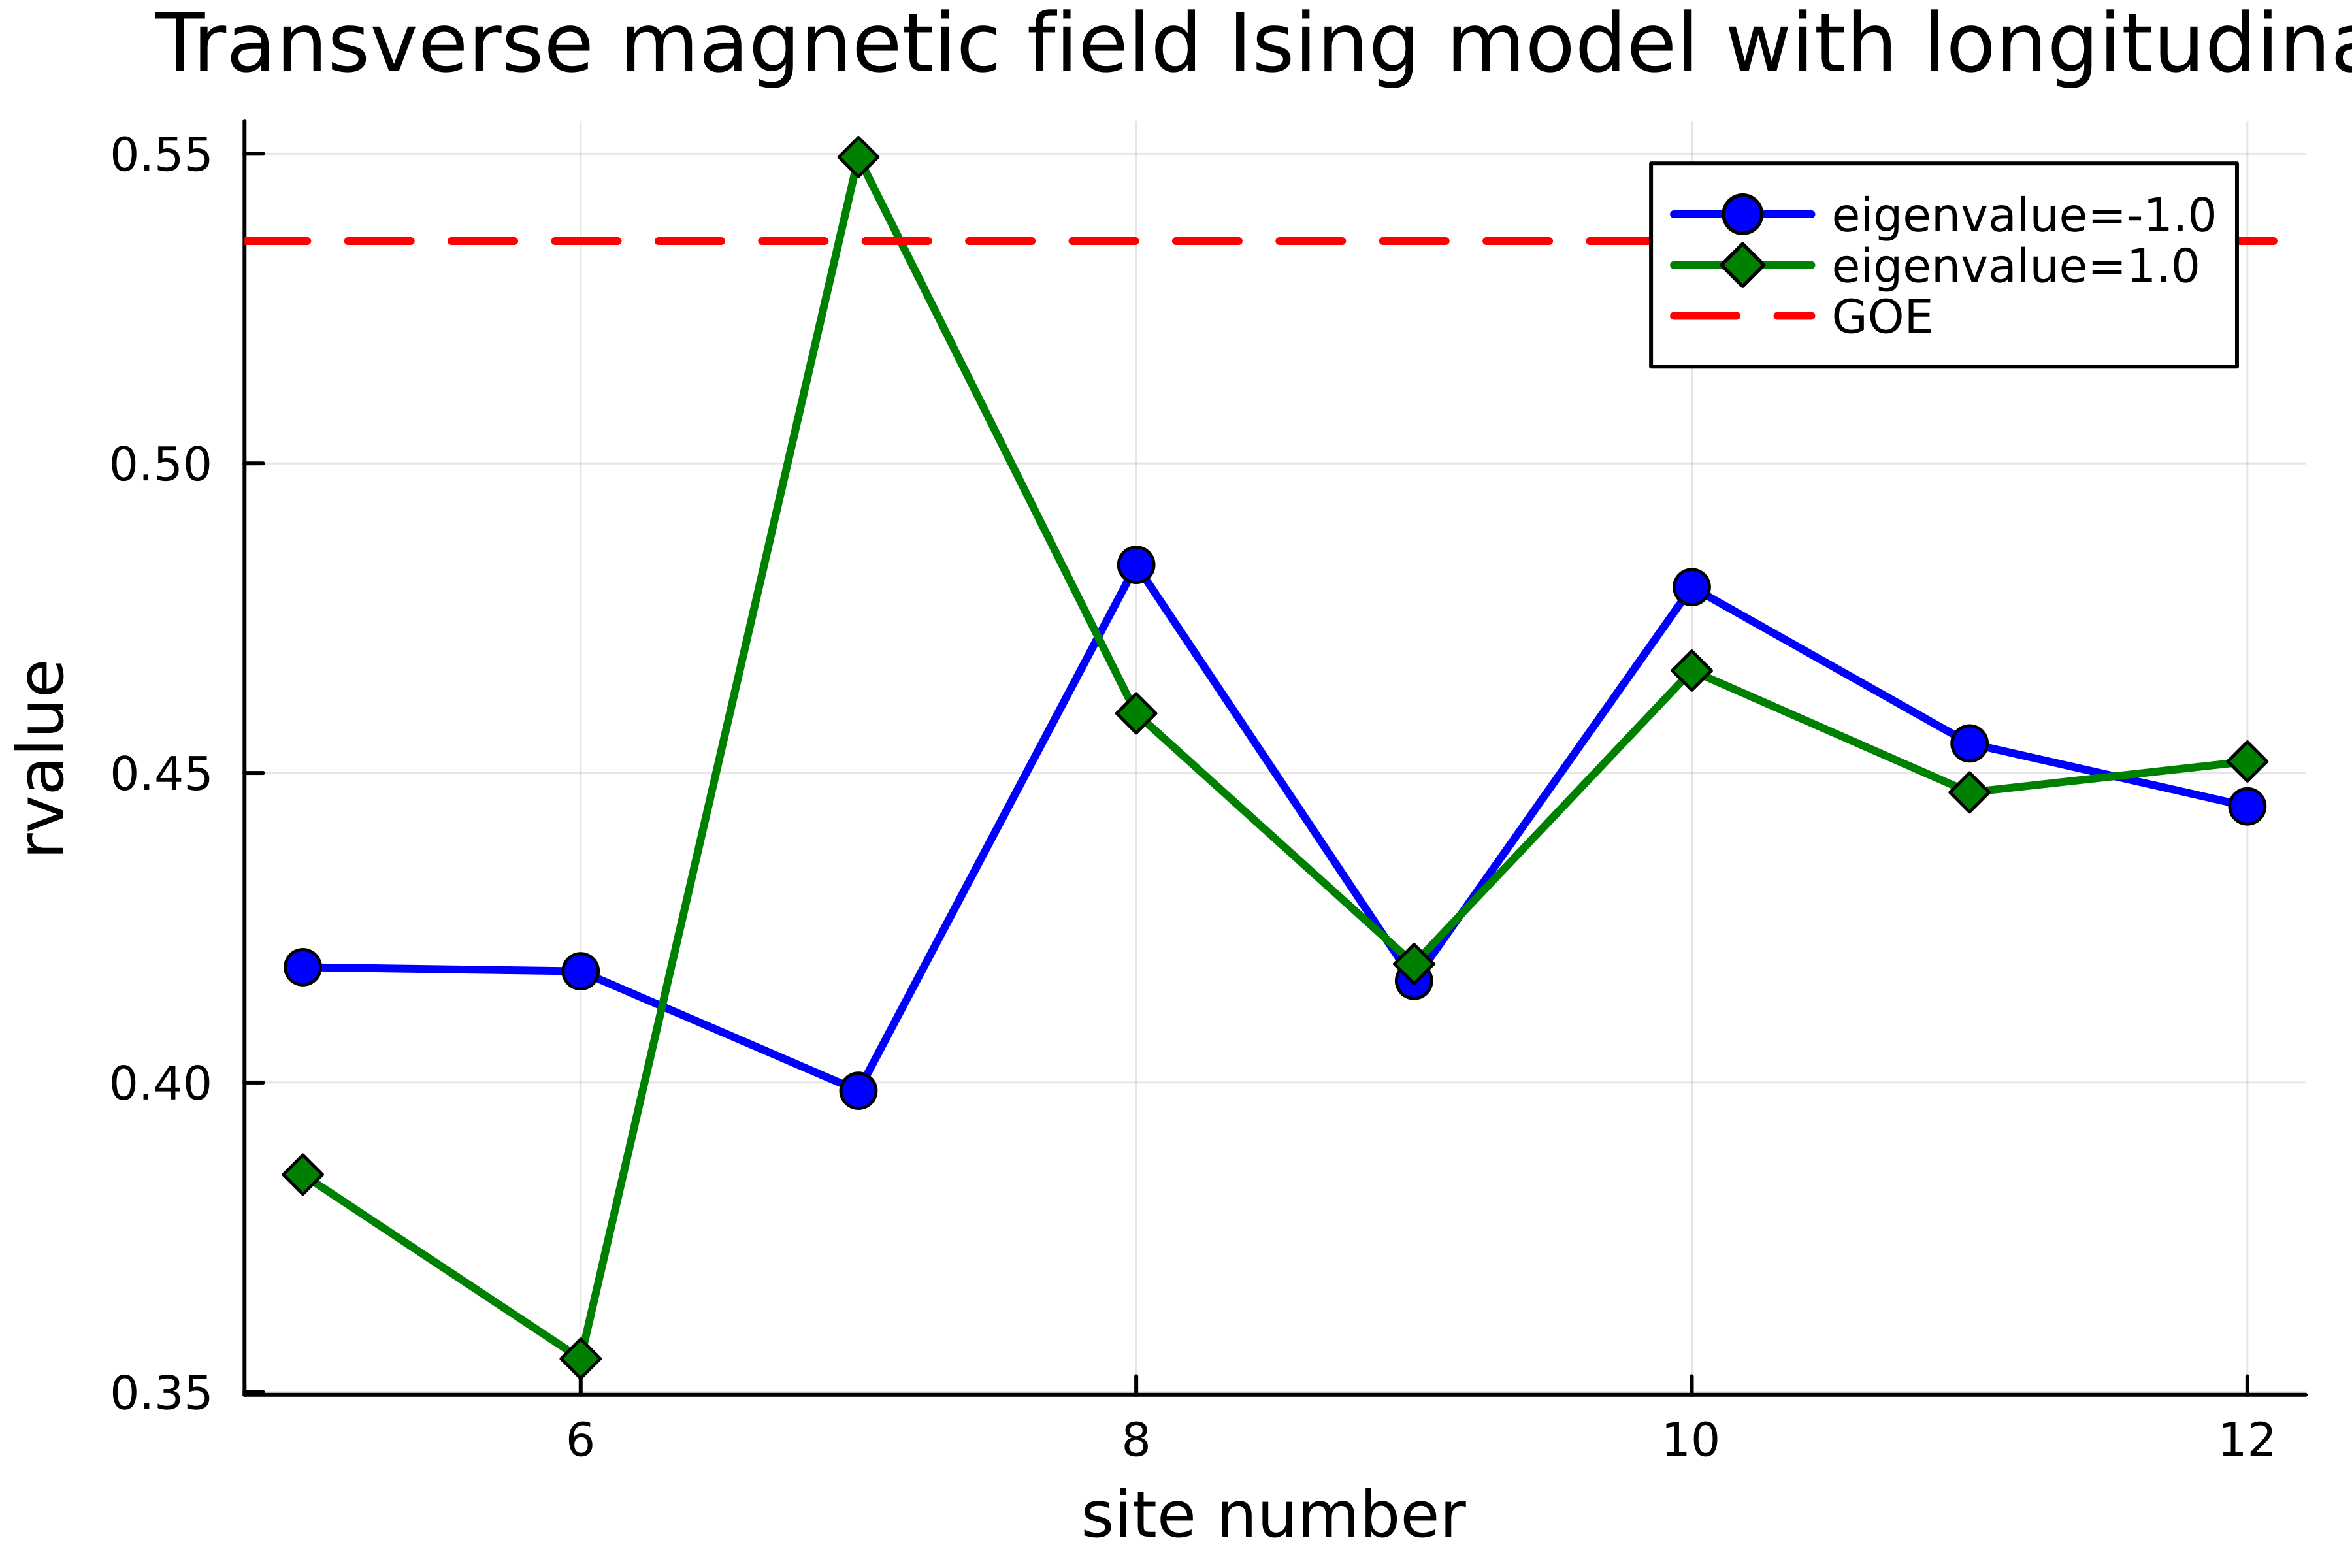
\includegraphics[width=150mm]{rvalue_transverse.png}
  \caption{縦磁場横磁場イジングモデル}
  \label{fig:rvalue_transverse}
\end{figure}
\subsection*{横磁場と縦磁場を加えたXXZモデル(開放端)--空間反転のみ}
\begin{gather}
  \hat{H}=J\sum_{i=1}^{N-1} \left(\frac{1}{2}(\hat{S}_i^+\hat{S}_{i+1}^- + \hat{S}_i^-\hat{S}_{i+1}^+) + \Delta\hat{S}_i^z\hat{S}_{i+1}^z\right)  - \frac{h}{2}\sum_{i=1}^{N} \left( \hat{S}_i^+ + \hat{S}_i^- \right) - v\sum_{i=1}^{N} \hat{S}_i^z\\
  \Delta=\sqrt{1.3},\frac{h}{J}=\sqrt{1.5},\frac{v}{J}=\sqrt{2}
\end{gather}
\begin{figure}[H]
  \centering
  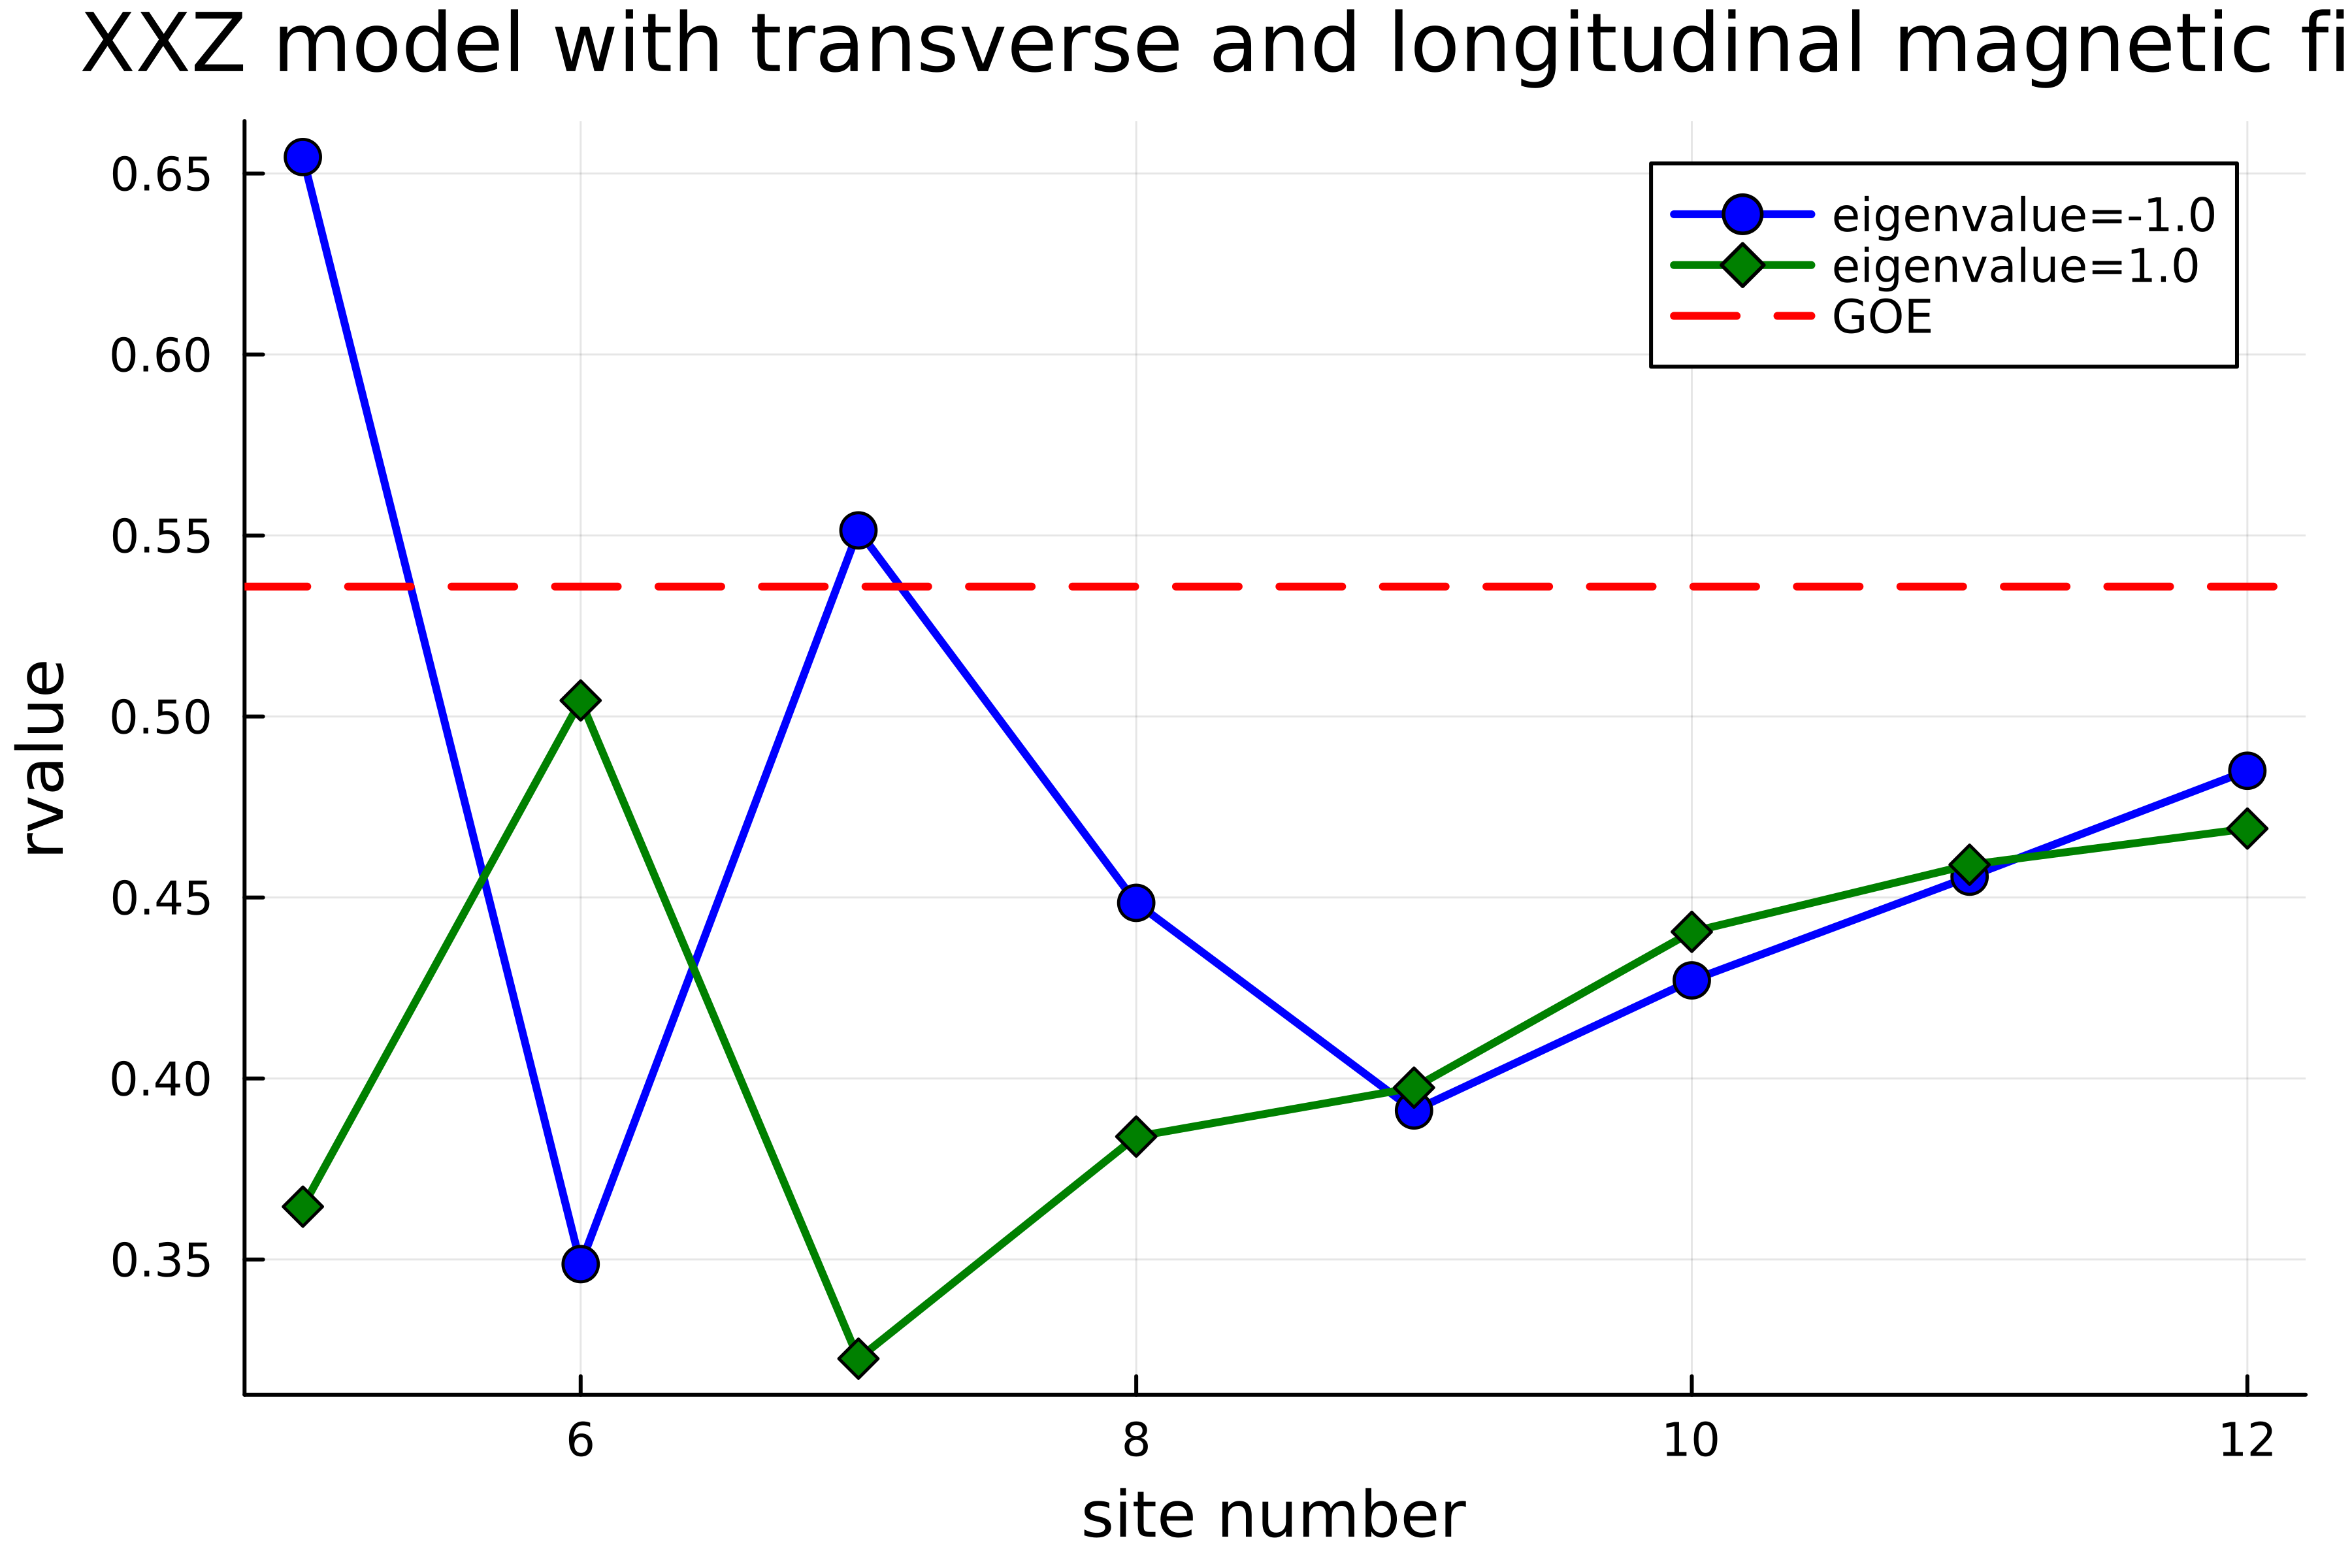
\includegraphics[width=150mm]{rvalue_xxz.png}
  \caption{横磁場と縦磁場を加えたXXZモデル}
  \label{fig:rvalue_xxz}
\end{figure}
どちらもあまり収束しておらず微妙な結果となっている。縮退しているかどうかの判定はfalseであり既約分解はできており、普通に対角化した場合と比べてもエネルギー固有値は等しいのでブロック対角化にも問題がないと思われる。\\
コードは以下のように書いた。
\begin{jllisting}
using .ExactDiag
using Plots
default(dpi=600)
x=Vector{Float64}()
y11=Vector{Float64}()
y12=Vector{Float64}()
y21=Vector{Float64}()
y22=Vector{Float64}()
for L in 5:12
  push!(x, L)
  init(2,L)
  hj = sqrt(1.5)
  vj = sqrt(2.0)
  Δ = sqrt(1.3)
  H1 = sum(j -> spin('z', j) * spin('z', j + 1), 1) - sum(j -> hj * spin('x', j)) - sum(j -> vj * spin('z', j))
  H2 = sum(j -> spin('x', j) * spin('x', j + 1) + spin('y', j) * spin('y', j + 1) + Δ * spin('z', j) * spin('z', j + 1),1) - sum(j -> hj * spin('x', j)) - sum(j -> vj * spin('z', j))
  dict1= block_diag1_rvalue(H1, site_flip(), true)
  push!(y11, dict1[-1.0 + 0.0im])
  push!(y12, dict1[1.0 + 0.0im])
  dict2= block_diag1_rvalue(H2, site_flip(), true)
  push!(y21, dict2[-1.0 + 0.0im])
  push!(y22, dict2[1.0 + 0.0im])
end
plot(x, y11, label="eigenvalue=-1.0", xlabel="site number", ylabel="rvalue", title="Transverse magnetic field Ising model with longitudinal magnetic field", legend=:topright, marker=:circle, markersize=5, linewidth=2, color=:blue)
plot!(x, y12, label="eigenvalue=1.0",marker=:diamond, markersize=5, linewidth=2, color=:green)
threshold = 4.0-2.0*sqrt(3.0)
hline!([threshold];
  label="GOE",
  linestyle=:dash, linewidth=2, color=:red)
cd(raw"\\wsl.localhost\Ubuntu\home\kokor\git\exact_diag")
savefig("rvalue_transverse1.png")
plot(x, y21, label="eigenvalue=-1.0", xlabel="site number", ylabel="rvalue", title="XXZ model with transverse and longitudinal magnetic field", legend=:topright, marker=:circle, markersize=5, linewidth=2, color=:blue)
plot!(x, y22, label="eigenvalue=1.0",marker=:diamond, markersize=5, linewidth=2, color=:green)
threshold = 4.0-2.0*sqrt(3.0)
hline!([threshold];
  label="GOE",
  linestyle=:dash, linewidth=2, color=:red)
cd(raw"\\wsl.localhost\Ubuntu\home\kokor\git\exact_diag")
savefig("rvalue_xxz1.png")
\end{jllisting}
\section{エンタングルメントエントロピーの計算}
\section{エンタングルメントエントロピーの計算結果}
\subsection*{縦磁場横磁場イジングモデル(開放端)—空間反転のみ}
\begin{gather}
  \hat{H}=J\sum_{i=1}^{N-1} \hat{S}_i^z\hat{S}_{i+1}^z - \frac{h}{2}\sum_{i=1}^{N} \left( \hat{S}_i^+ + \hat{S}_i^- \right) - v\sum_{i=1}^{N} \hat{S}_i^z\\
  \frac{h}{J}=\sqrt{1.5},\frac{v}{J}=\sqrt{2.0}
\end{gather}
\begin{figure}[H]
  \centering
  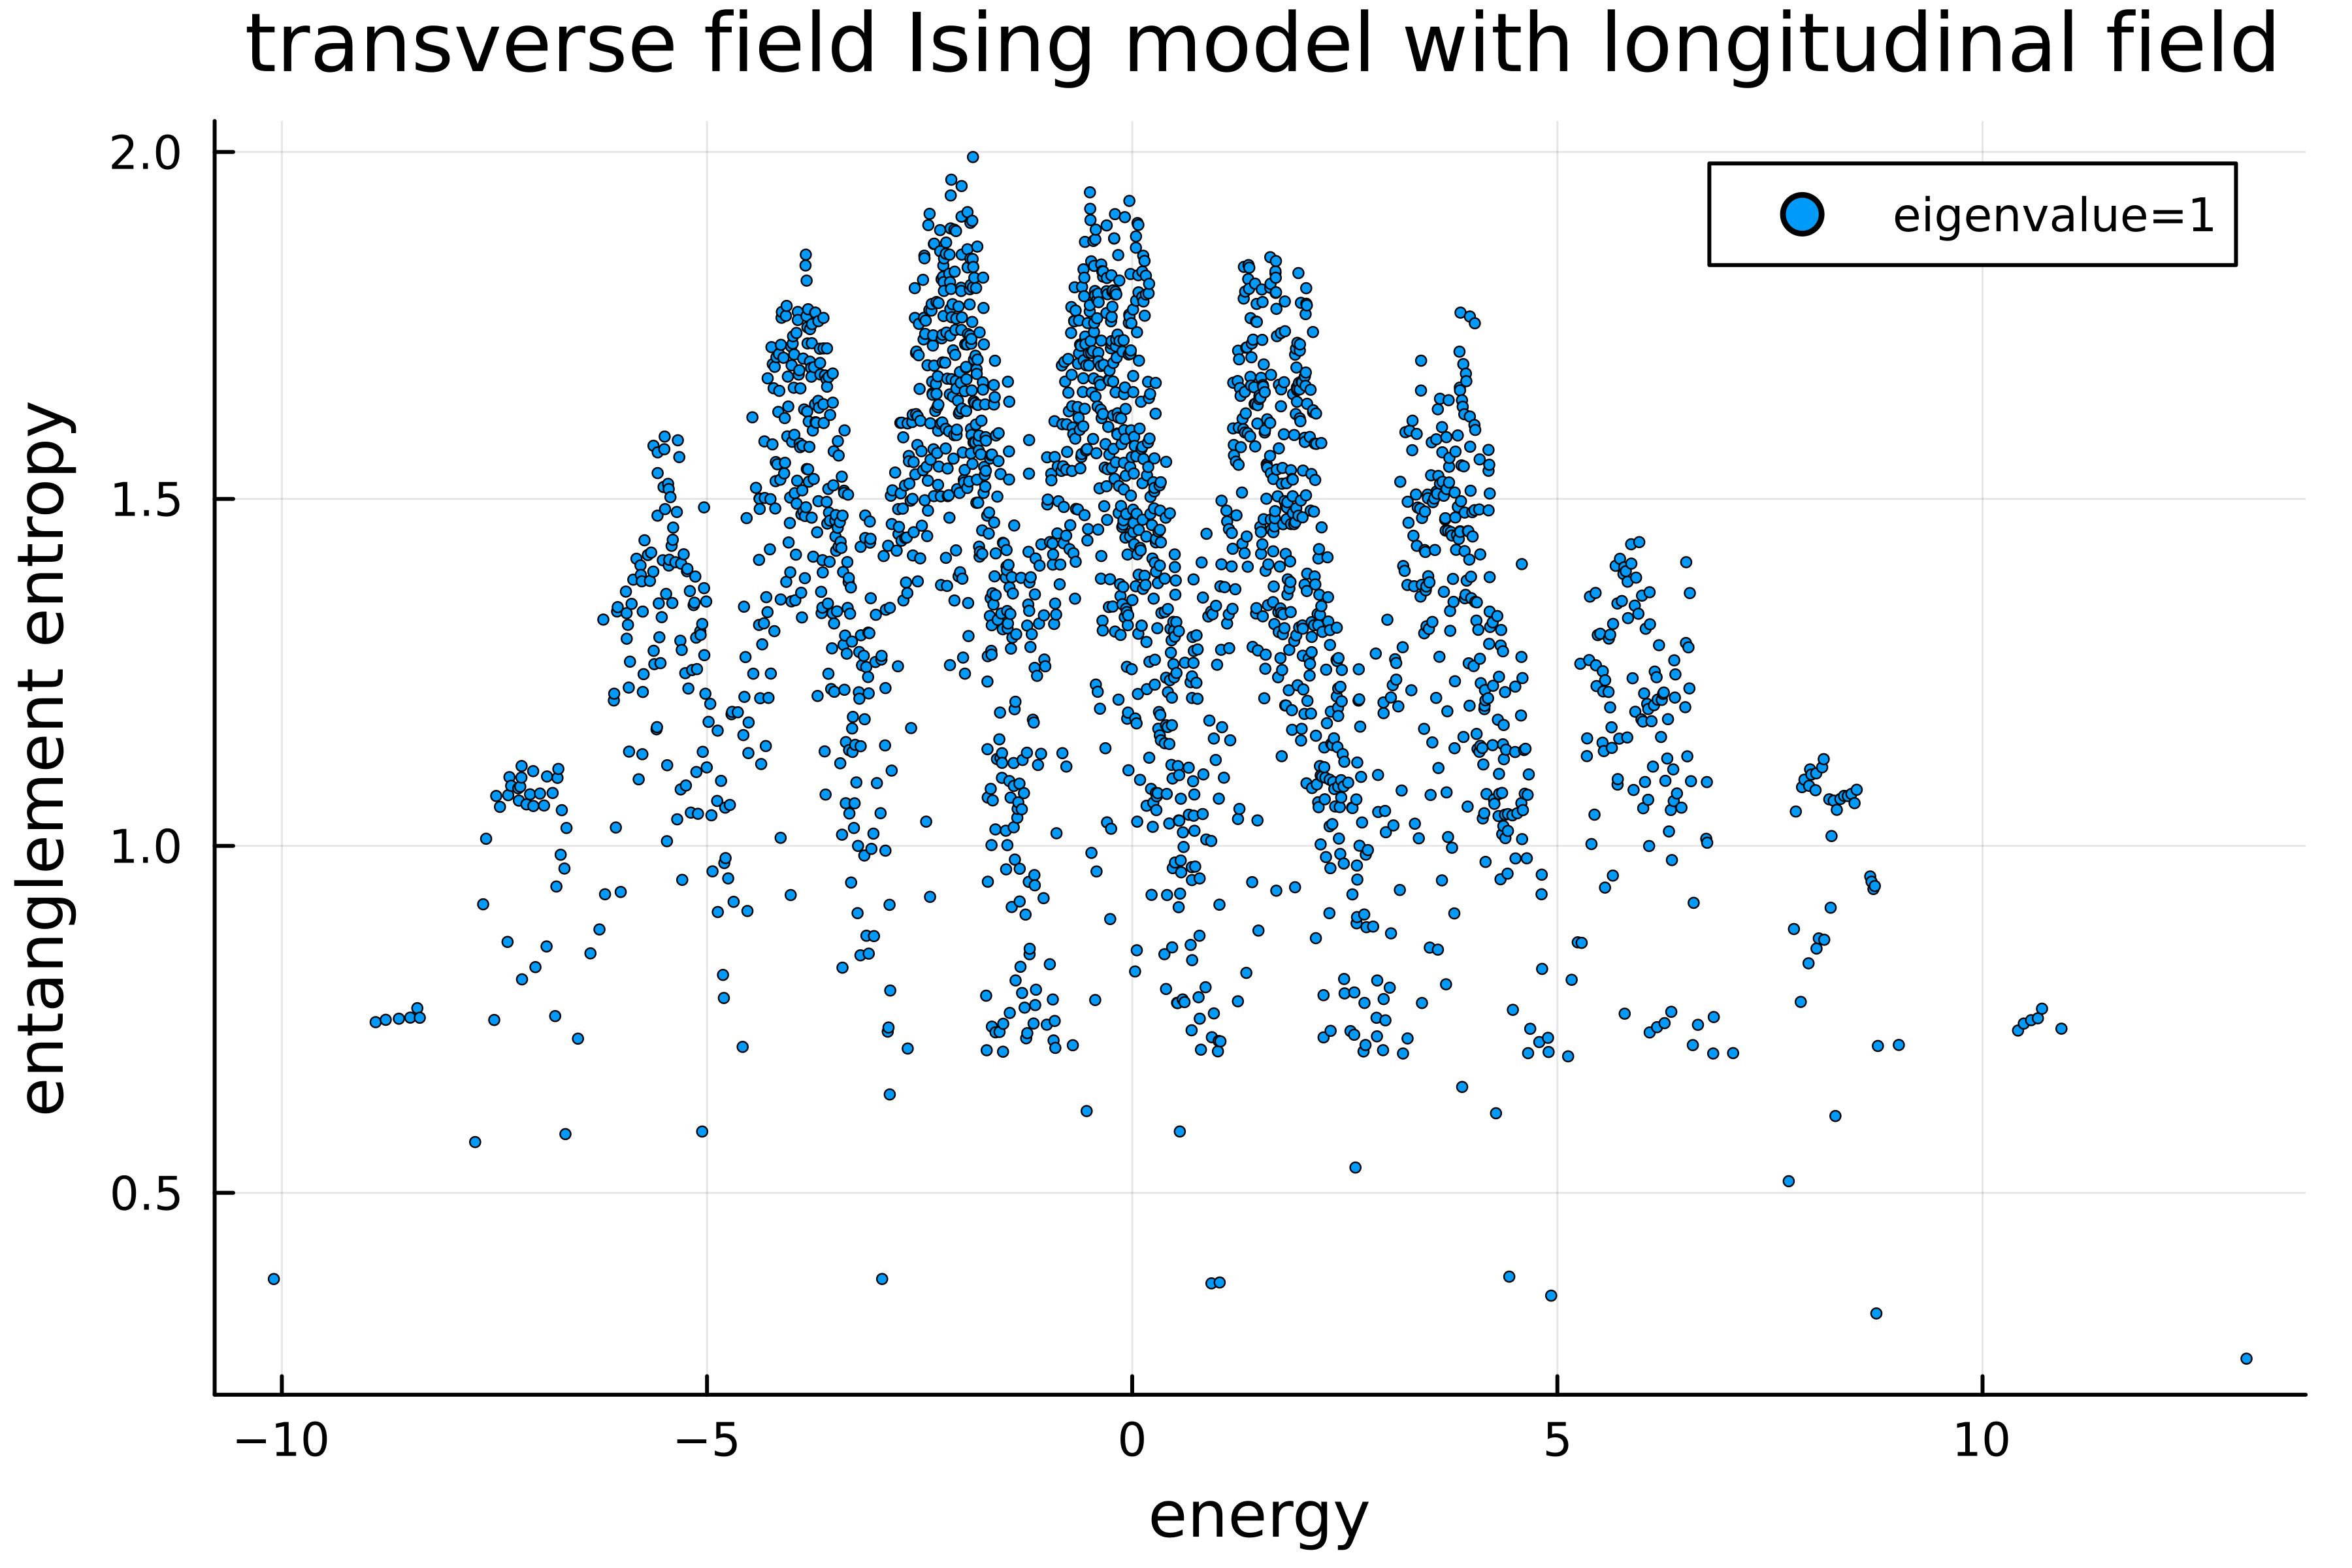
\includegraphics[width=150mm]{entropy_siteflip.png}
  \caption{縦磁場を入れた横磁場イジングモデル}
  \label{fig:entropy_siteflip}
\end{figure}
ここで、$\frac{h}{J}=10000$とすると。
\begin{figure}[H]
  \centering
  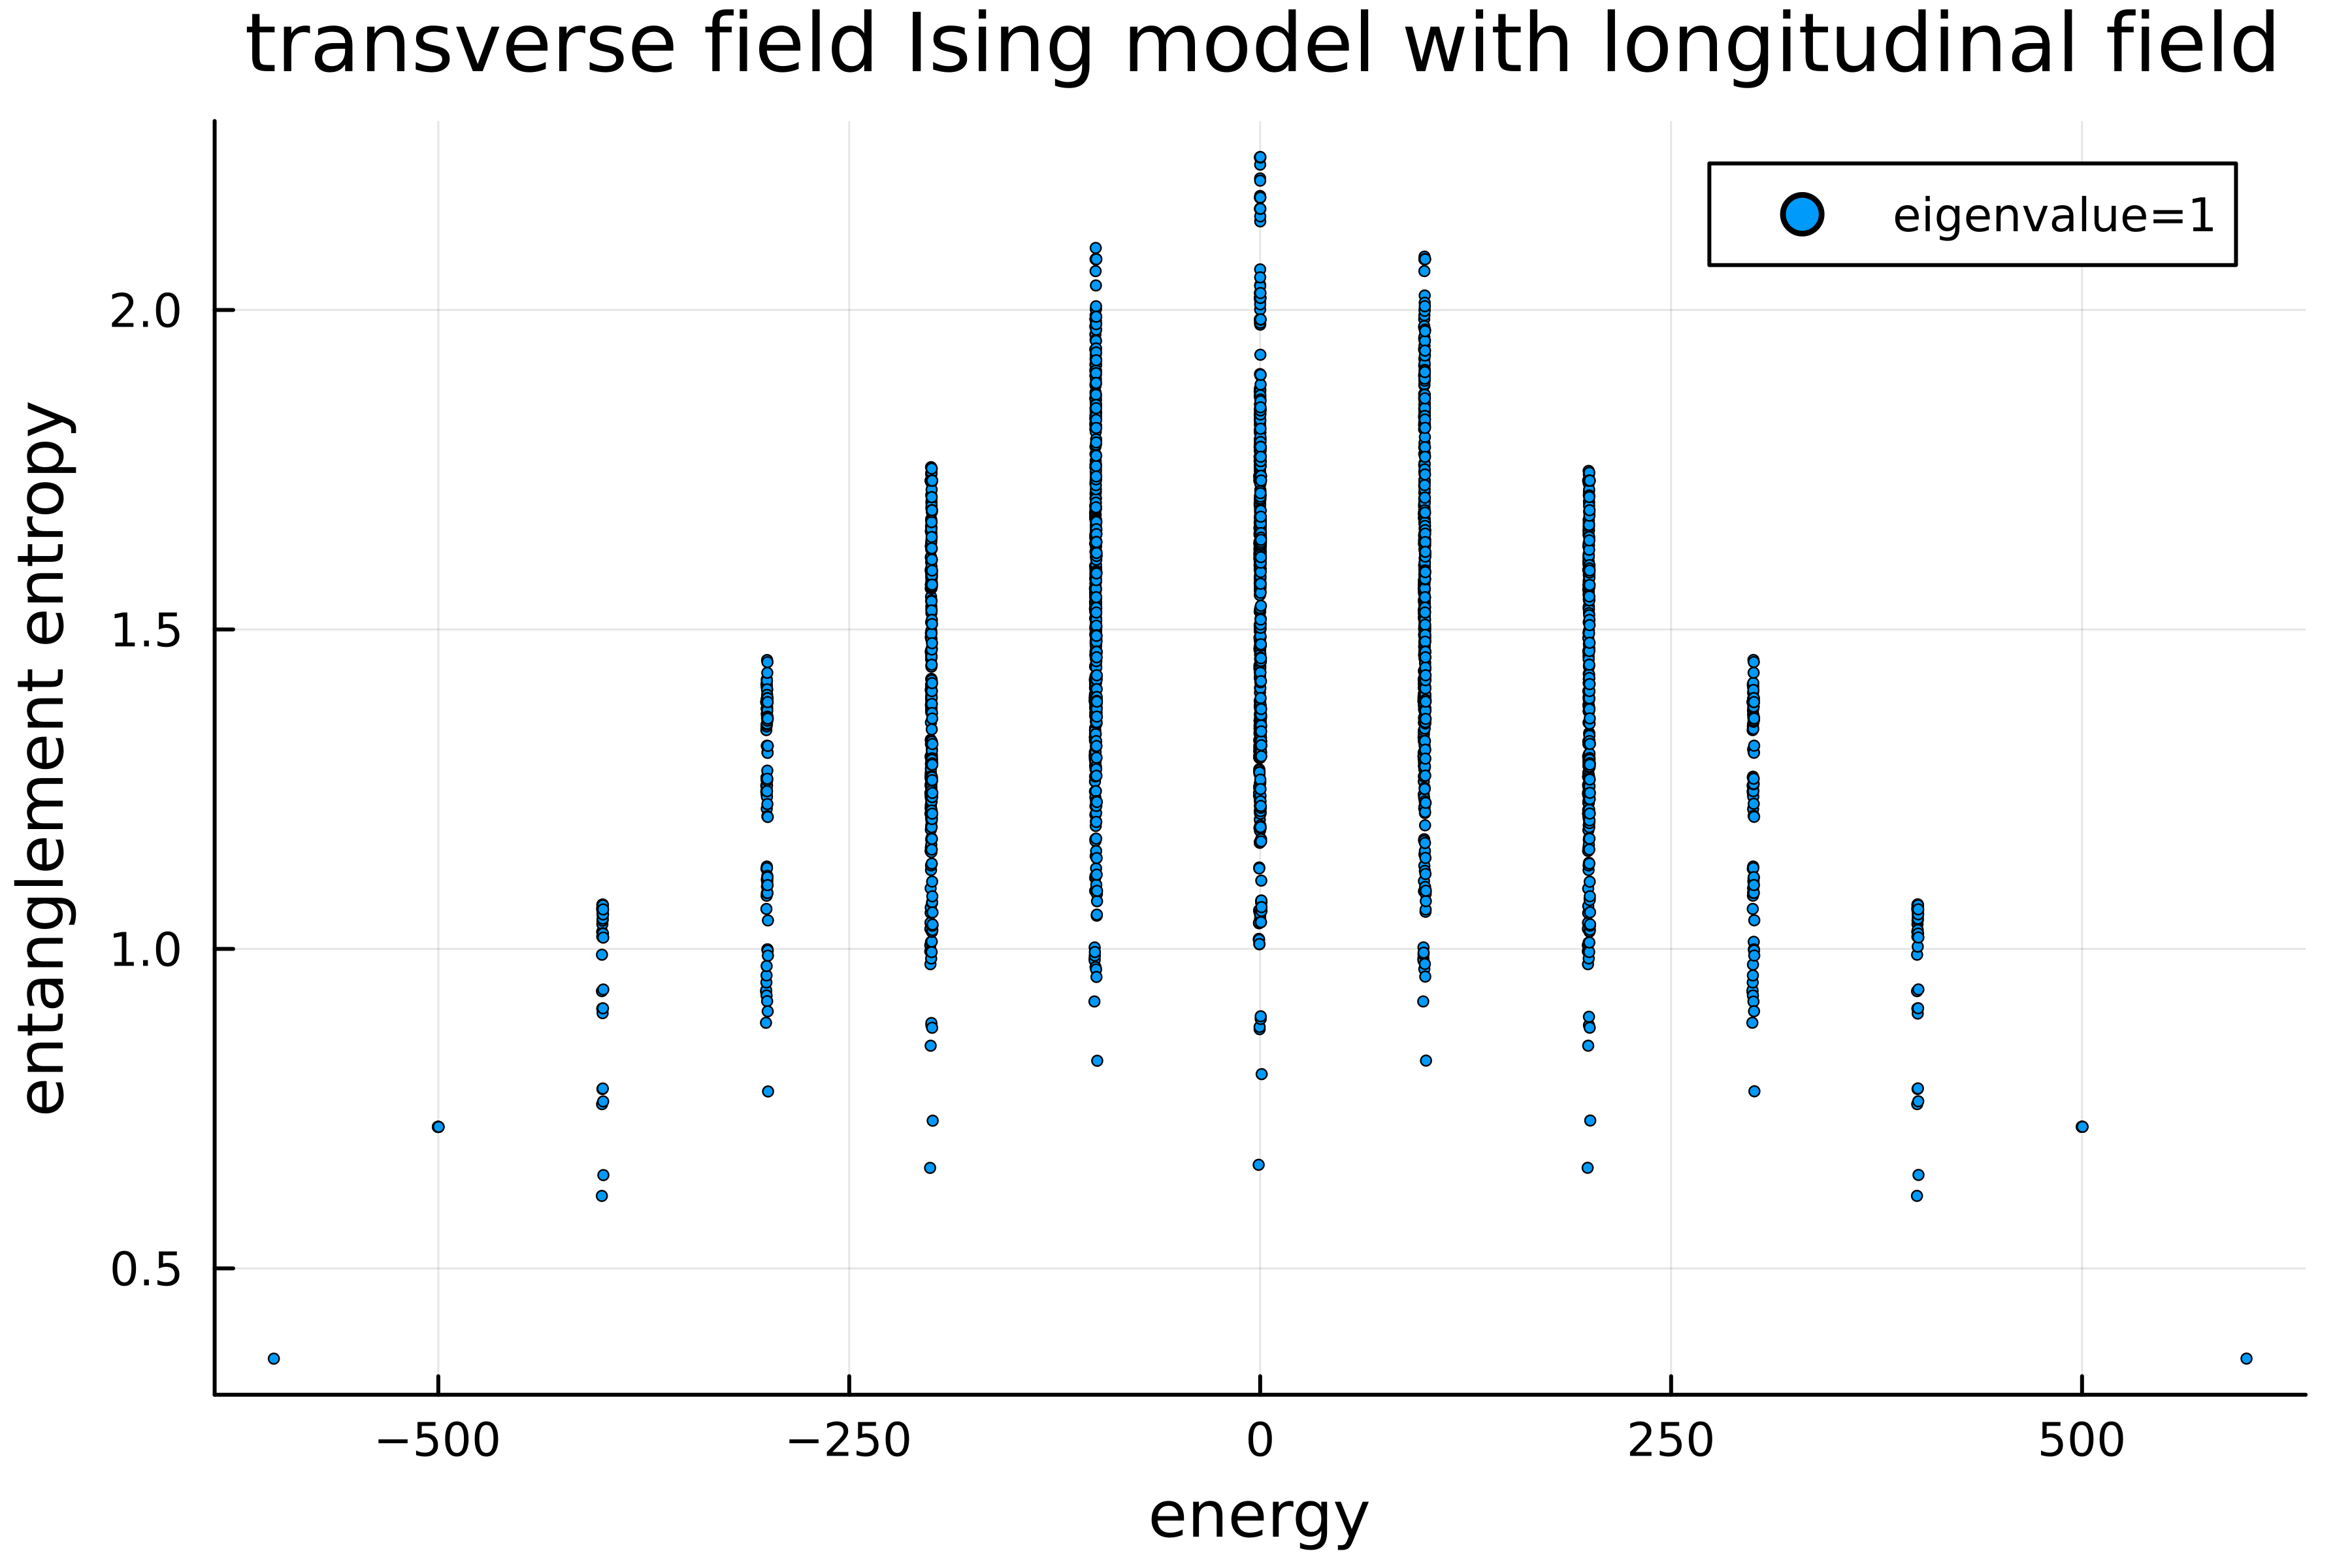
\includegraphics[width=150mm]{entropy_hjmax.png}
  \caption{縦磁場を入れた横磁場イジングモデル}
  \label{fig:entropy_hjmax}
\end{figure}
このようにほぼ縮退しており、x方向のスピンにより分解されている。\\
\subsection*{横磁場イジングモデル(開放端)—空間反転のみ}
\begin{gather}
  \hat{H}=J\sum_{i=1}^{N-2} \hat{S}_i^z\hat{S}_{i+1}^z + k\hat{S}_{N-1}^z\hat{S}_{N}^z - \frac{h}{2}\sum_{i=1}^{N} \left( \hat{S}_i^+ + \hat{S}_i^- \right)\\
  \frac{h}{J}=\sqrt{1.5},\frac{k}{J}=\sqrt{2.5}
\end{gather}
\begin{figure}[H]
  \centering
  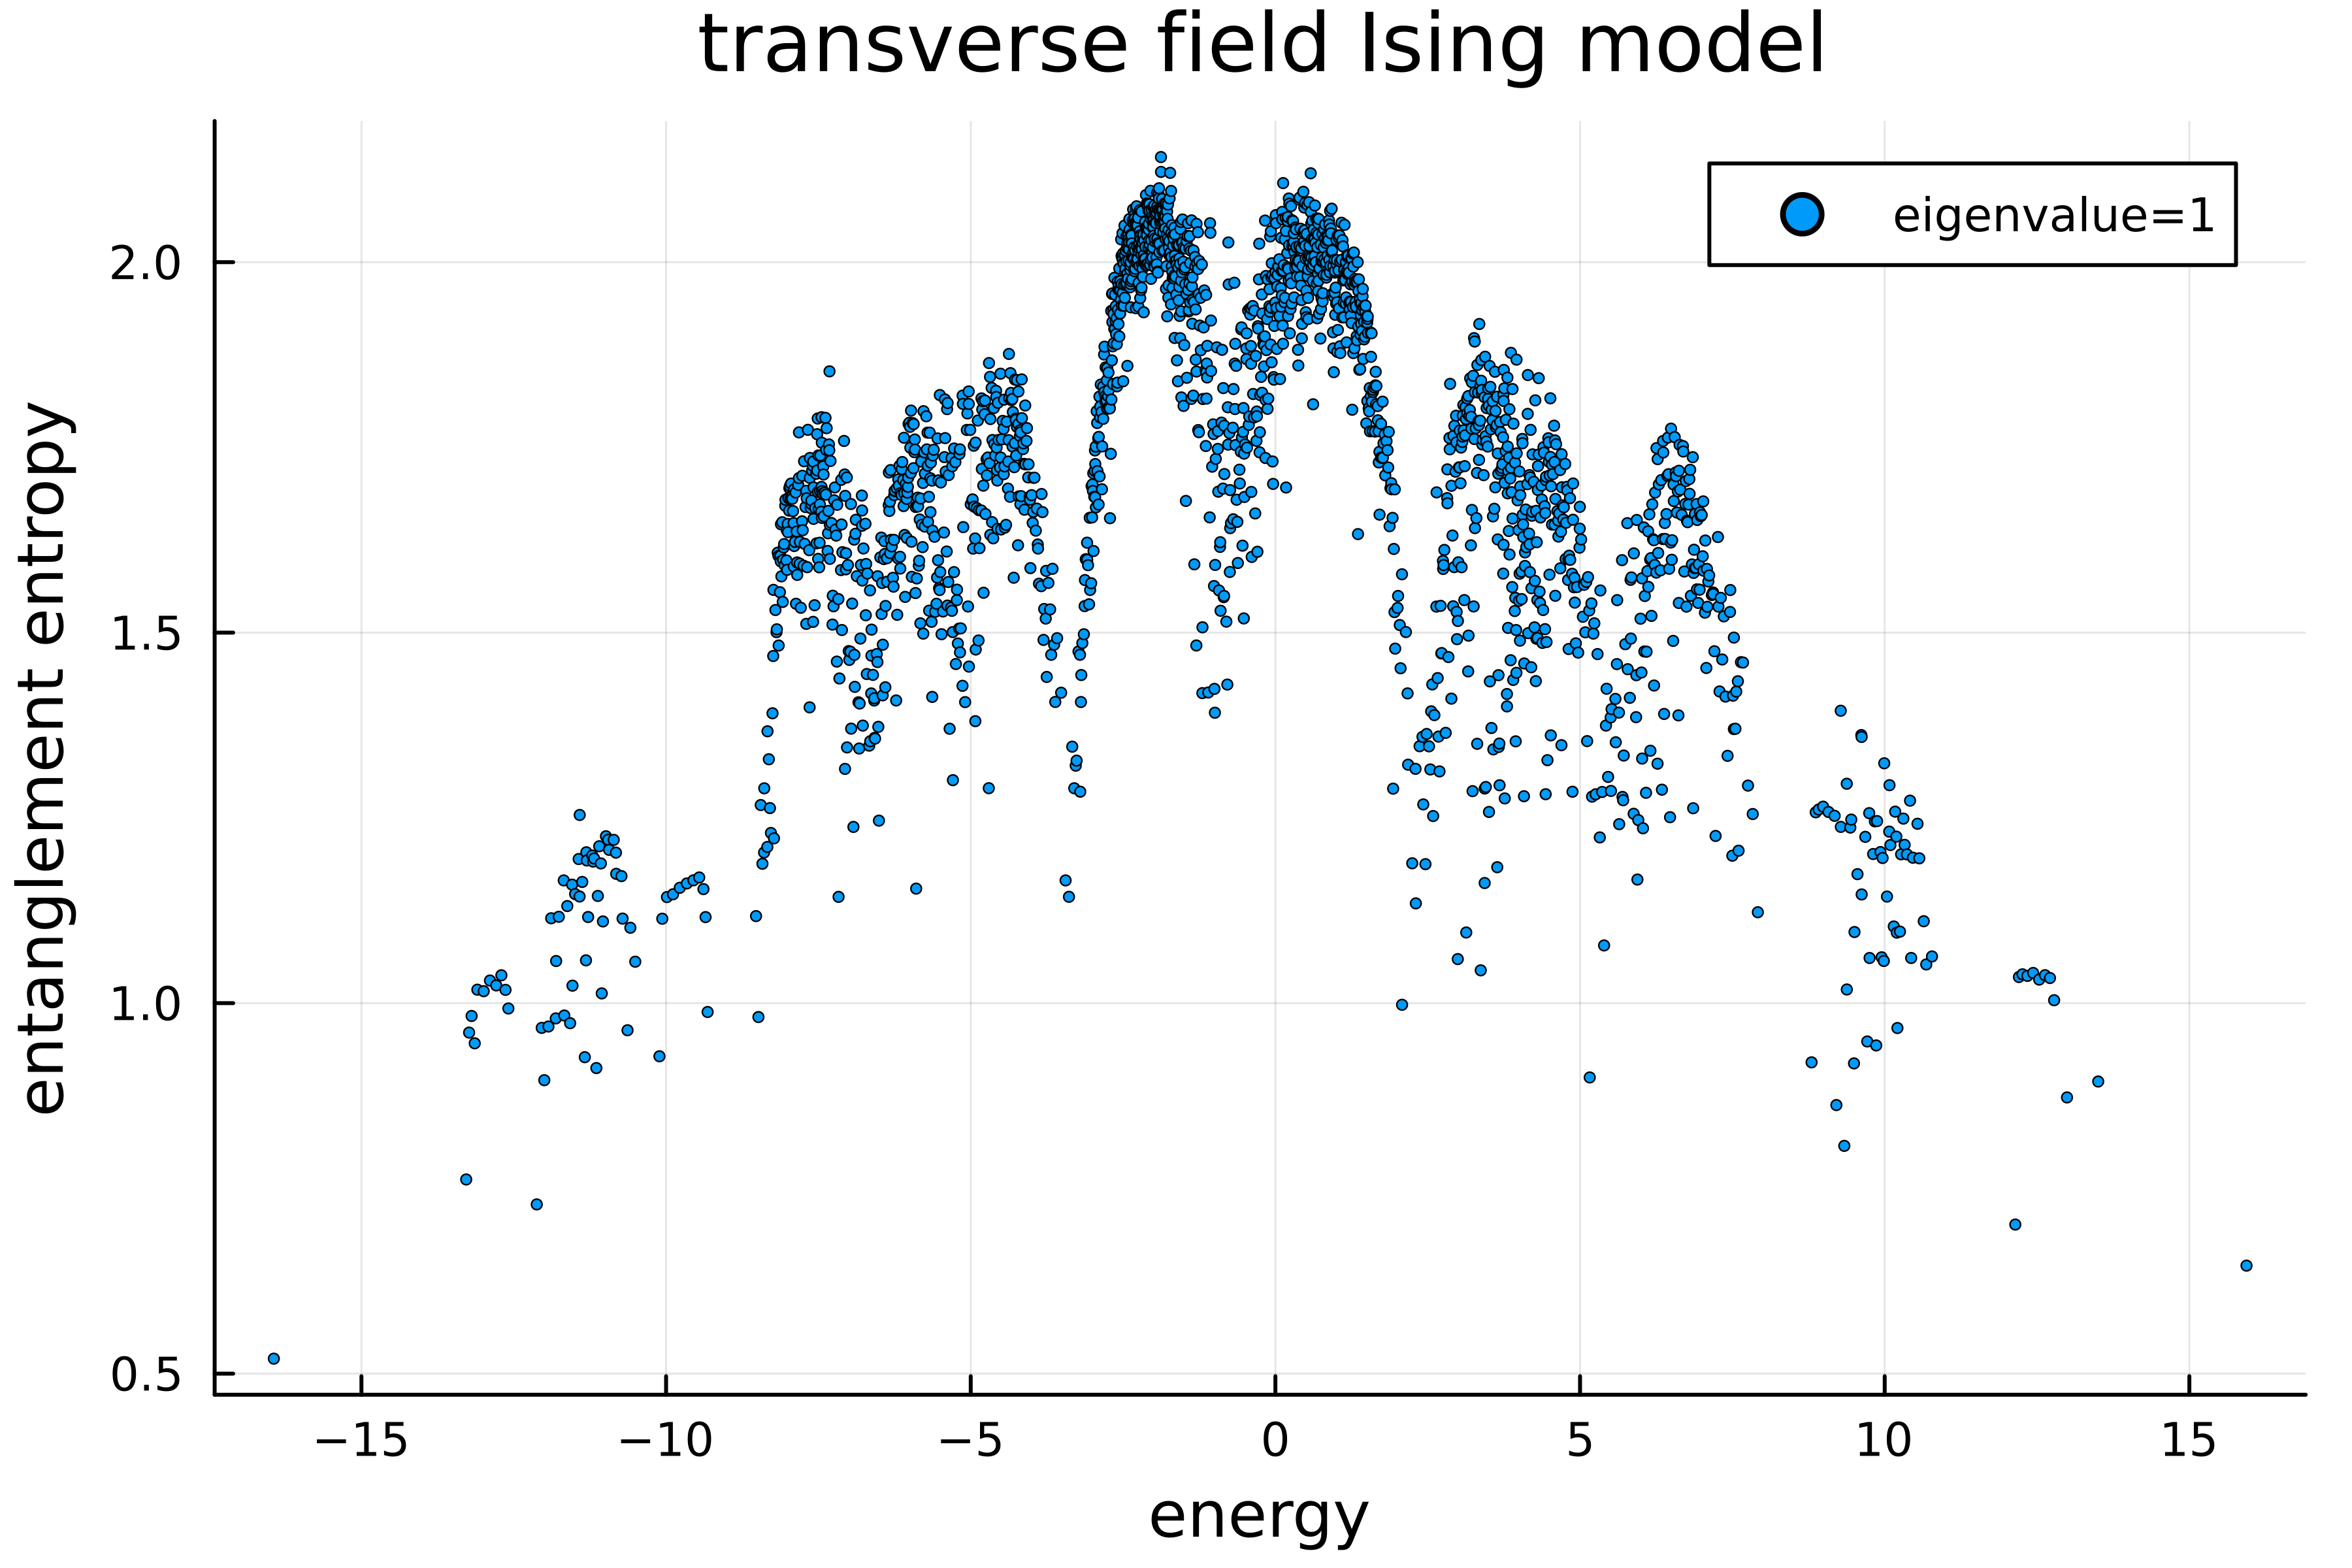
\includegraphics[width=150mm]{entropy_spinflip.png}
  \caption{横磁場イジングモデル}
  \label{fig:entropy_spinflip}
\end{figure}

\subsection*{サイン関数による縦磁場勾配を加えたXXZ模型(開放端)—U(1)対称性のみ}
\begin{gather}
  \hat{H}=J\sum_{i=1}^{N-1} \left(\frac{1}{2}(\hat{S}_i^+\hat{S}_{i+1}^- + \hat{S}_i^-\hat{S}_{i+1}^+) + \Delta\hat{S}_i^z\hat{S}_{i+1}^z\right) + v\sum_{i=1}^{N} \sin(i)\hat{S}_i^z\\
  \Delta=\sqrt{1.3},\frac{v}{J}=\sqrt{2}
\end{gather}
\begin{figure}[H]
  \centering
  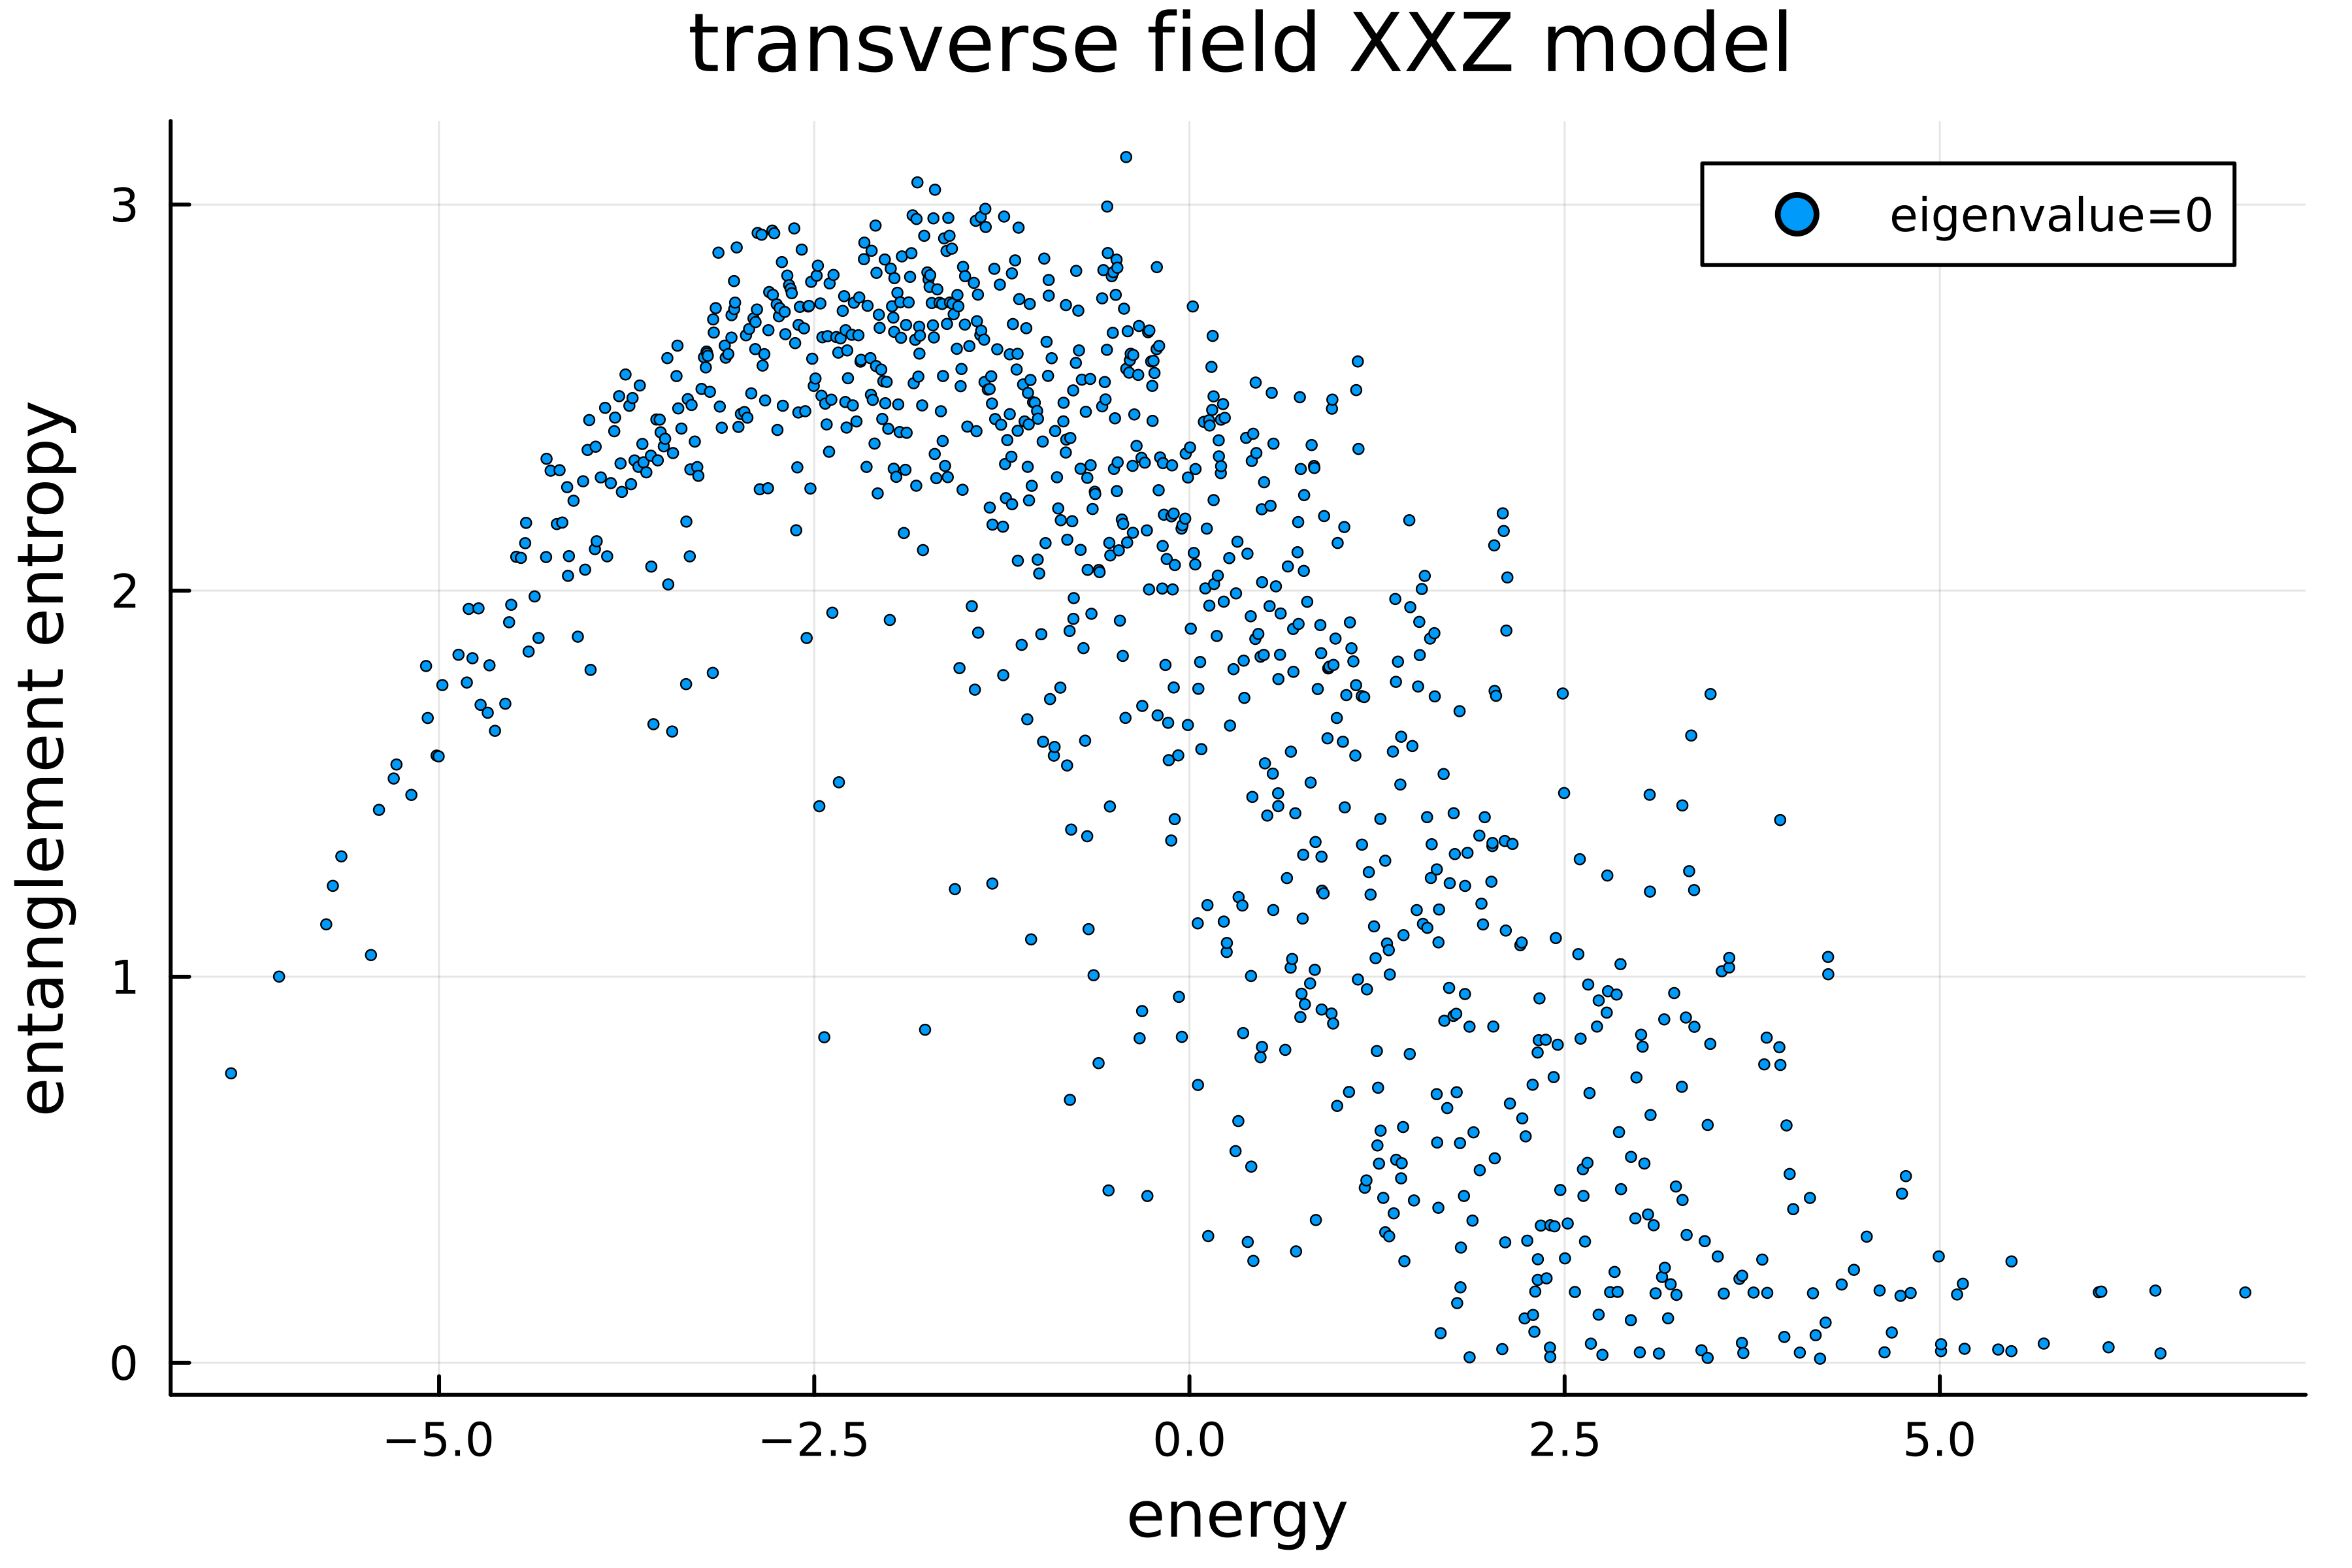
\includegraphics[width=150mm]{entropy_xxz.png}
  \caption{縦磁場を入れたXXZ模型}
  \label{fig:entropy_xxz}
\end{figure}
\begin{jllisting}
using .ExactDiag
using Plots
default(dpi=600)
x1=Vector{Float64}()
x2=Vector{Float64}()
x3=Vector{Float64}()
x4=Vector{Float64}()
y1=Vector{Float64}()
y2=Vector{Float64}()
y3=Vector{Float64}()
y4=Vector{Float64}()
L = 12
init(2,L)
hj = sqrt(1.5)
vj = sqrt(2.0)
Δ = sqrt(1.3)
kj = sqrt(2.5)
H1 = sum(j -> spin('z', j) * spin('z', j + 1), 1) - sum(j -> hj * spin('x', j)) - sum(j -> vj * spin('z', j))
H2 = sum(j -> spin('z', j) * spin('z', j + 1), 2) + kj * spin('z', 1) * spin('z', 2) - sum(j -> hj * spin('x', j))
H3 = sum(j -> spin('x', j) * spin('x', j + 1) + spin('y', j) * spin('y', j + 1) + Δ * spin('z', j) * spin('z', j + 1),1) - sum(j -> vj * sin(j) * spin('z', j))
H4 = sum(j -> spin('z', j) * spin('z', j + 1), 1) - sum(j -> 10000.0 * spin('x', j)) - sum(j -> vj * spin('z', j))
x1, y1 = block_diag1_entanglement_entropy(H1, site_flip(), 1.0 + 0.0im)
x2, y2 = block_diag1_entanglement_entropy(H2, spin_flip(), 1.0 + 0.0im)
x3,y3 = block_diag1_entanglement_entropy(H3, S_z(), 0.0 + 0.0im)
x4,y4 = block_diag1_entanglement_entropy(H4, site_flip(), 1.0 + 0.0im)
scatter(x1, y1;
  label="eigenvalue=1",
  xlabel="energy",
  ylabel="entanglement entropy",
  title="transverse field Ising model with longitudinal field",
  markersize=1.5, markerstrokewidth=0.5)
cd(raw"\\wsl.localhost\Ubuntu\home\kokor\git\exact_diag")
savefig("entropy_siteflip1.png")
scatter(x2, y2;
  label="eigenvalue=1",
  xlabel="energy",
  ylabel="entanglement entropy",
  title="transverse field Ising model",
  markersize=1.5, markerstrokewidth=0.5)
cd(raw"\\wsl.localhost\Ubuntu\home\kokor\git\exact_diag")
savefig("entropy_spinflip.png")
scatter(x3, y3;
  label="eigenvalue=0",
  xlabel="energy",
  ylabel="entanglement entropy",
  title="transverse field XXZ model",
  markersize=1.5, markerstrokewidth=0.5)
cd(raw"\\wsl.localhost\Ubuntu\home\kokor\git\exact_diag")
savefig("entropy_xxz.png")
scatter(x4, y4;
  label="eigenvalue=1",
  xlabel="energy",
  ylabel="entanglement entropy",
  title="transverse field Ising model with longitudinal field",
  markersize=1.5, markerstrokewidth=0.5)
cd(raw"\\wsl.localhost\Ubuntu\home\kokor\git\exact_diag")
savefig("entropy_hjmax.png")
\end{jllisting}
このようなコードを用いて計算した。\\


\end{document}